\باب{تفرق}
گزشتہ باب میں ہم نے دیکھا کہ کسی نقطہ پر سیکنٹ کی ڈھلوان کی حد کو اس نقطے پر منحنی کی ڈھلوان کہتے ہیں۔ یہ حد، جس کو تفرق کہتے ہیں، تفاعل تبدیل ہونے کی شرح کی ناپ ہے جو احصاء میں اہم ترین تصورات میں سے ایک ہے۔تفرق کو سائنس، معاشیات اور دیگر شعبوں میں بہت زیادہ استعمال کیا جاتا ہے جہاں سمتی رفتار اور اسراع کا حساب، مشین کی کارکردگی سمجھنے، وغیرہ کے لئے اس کو استعمال میں لایا جاتا ہے۔تفرق کو حد سے تلاش کرنا مشکل کام ہے۔اس باب میں تفرق حاصل کرنے کے طریقوں پر غور کیا جائے گا۔ 

\حصہ{تفاعل کا تفرق}
گزشتہ باب کے آخر میں ہم نے نقطہ \عددی{x=x_0} پر منحنی \عددی{y=f(x)} کی ڈھلوان \عددی{m} کی درج ذیل تعریف پیش کی۔
\begin{align*}
m=\lim_{h\to 0}\frac{f(x_0+h)-f(x_0)}{h}
\end{align*} 
اس حد کو، بشرطیکہ یہ موجود ہو، \عددی{x_0} پر \عددی{f} کا تفرق کہتے ہیں۔اس حصے میں \عددی{f} کی دائرہ کار میں ہر نقطے پر \عددی{f} کی ڈھلوان پر  بطور تفاعل غور کیا جائے گا۔

\ابتدا{تعریف}
متغیر \عددی{x} کے لحاظ سے تفاعل \عددی{f} کا \اصطلاح{تفرق}\فرہنگ{تفرق}\حاشیہب{derivative}\فرہنگ{derivative} درج ذیل  تفاعل \عددی{f'} ہے، بشرطیکہ یہ حد موجود ہو۔
\begin{align*}
f'(x)=\lim_{h\to 0}\frac{f(x+h)-f(x)}{h}
\end{align*}
\انتہا{تعریف}
%===========================

\عددی{f'} کا دائرہ کار، نقطوں کا وہ سلسلہ جہاں یہ حد موجود ہو، تفاعل \عددی{f} کے دائرہ کار سے کم ہو سکتا ہے۔ اگر \عددی{f'(x)} موجود ہو تب ہم کہتے ہیں کہ \عددی{x} پر \عددی{f} کا \اصطلاح{تفرق} پایا جاتا ہے یا کہ \عددی{x} پر \عددی{f} \اصطلاح{قابل تفرق}\فرہنگ{تفرق!قابل}\حاشیہب{differentiable}\فرہنگ{differentiable} ہے۔

\جزوحصہء{علامتیت}
تفاعل \عددی{y=f(x)} کی تفرق کو ظاہر کرنے کے کئی طریقے رائج ہیں۔\عددی{f'(x)} کے علاوہ درج ذیل علامتیں کافی مقبول ہیں۔
\begin{description}
\جزو{$y'$}
یہ مختصر علامت ہے جو غیر تابع متغیر کی نشاندہی نہیں کرتی ہے۔
\جزو{$\tfrac{\dif y}{\dif x}$}
یہ علامت دونوں متغیرات کی نشاندہی کرتی ہے اور تفرق کو \عددی{\dif} سے ظاہر کرتی ہے۔  
\جزو{$\tfrac{\dif f}{\dif x}$}
یہ علامت تفاعل کا نام واضح کرتی ہے۔
\جزو{$\tfrac{\dif}{\dif x} f(x)$}
اس علامت سے ظاہر ہوتا ہے کہ تفرق کا عمل \عددی{f} پر لاگو کیا جاتا ہے (شکل \حوالہ{شکل_تفرق_ڈبہ_صورت})۔
\جزو{$D_xf$}
یہ تفرقی عامل ہے۔
\جزو{$\dot{y}$} 
نیوٹن اس علامت کو استعمال کرتے تھے جو اب وقتی تفرق کو ظاہر کرنے کے لئے استعمال کیا جاتا ہے۔
\end{description} 

ہم \عددی{\tfrac{\dif y}{\dif x}} کو "\عددی{x} کے لحاظ سے \عددی{y} کو تفرق" پڑھتے ہیں۔اسی طرح \عددی{\tfrac{\dif f}{\dif x}} اور \عددی{\tfrac{\dif}{\dif x}f(x)} کو "\عددی{x} کے لحاظ سے \عددی{f} کا تفرق" پڑھا جاتا ہے۔
\begin{figure}
\centering
\begin{tikzpicture}
\draw(0,0) rectangle ++(2,1);
\draw[latex-](0,0.5)--++(-2,0)node[pos=0.5,above,align=center]{\RL{داخلی تفاعل}\\  $y=f(x)$};
\draw[-latex](2,0.5)--++(2,0)node[pos=0.5,above,align=center]{\RL{خارجی تفرق}\\ $y'=\tfrac{\dif f}{\dif x}$};
\draw(1,0.5)node[align=center]{\RL{عمل تفرق}\\ $\tfrac{\dif}{\dif x}$};
\end{tikzpicture}
\caption{تفرق کے عمل کی ڈبہ صورت}
\label{شکل_تفرق_ڈبہ_صورت}
\end{figure}

\جزوحصہء{تفرق کی تعریف سے تفرق کا حصول}
مثال \حوالہ{مثال_حد_سیدھا_خط_الف} اور مثال \حوالہ{مثال_حد_ڈھلوان} میں تفاعل \عددی{y=mx+b} اور \عددی{y=\tfrac{1}{x}} کے تفرق کو تعریف سے حاصل کرنا دکھایا گیا۔مثال \حوالہ{مثال_حد_سیدھا_خط_الف} میں 
\begin{align*}
\frac{\dif}{\dif x}(mx+b)=m
\end{align*}
اور   مثال \حوالہ{مثال_حد_ڈھلوان} میں
\begin{align}
\frac{\dif}{\dif x}\big(\frac{1}{x}\big)=-\frac{1}{x^2}
\end{align}
حاصل کیا گیا۔

\موٹا{تفرق کی تعریف سے  تفرق کے حاصل کے اقدام} 
\begin{enumerate}[1.]
\item
\عددی{f(x)} اور \عددی{f(x+h)} لکھیں۔
\item
درج ذیل تفریقی حاصل تقسیم کو پھیلا کر اس کی سادہ ترین صورت حاصل کریں۔
\begin{align*}
\frac{f(x+h)-f(x)}{h}
\end{align*}
\item
سادہ ترین حاصل تقسیم سے \عددی{f'(x)} حاصل کرنے کی خاطر درج ذیل حد تلاش کریں۔
\begin{align*}
f'(x)=\lim_{h\to 0}\frac{f(x+h)-f(x)}{h}
\end{align*}
\end{enumerate}

مزید دو مثال درج ذیل ہیں۔

\ابتدا{مثال}\شناخت{مثال_تفرق_حصول_بذریعہ_تعریف_الف}
\begin{enumerate}[a.]
\item
\عددی{f(x)=\tfrac{x}{x-1}} کو تفرق کریں۔
\item
تفاعل \عددی{y=f(x)} کی ڈھلوان کس نقطے پر \عددی{-1} کے برابر ہے؟
\end{enumerate}
حل:\quad  (ا) \quad  ہم مذکورہ بالا تین اقدام استعمال کرتے ہوئے تعریف سے تفرق حاصل کرتے ہیں۔\\
\موٹا{پہلا قدم:} یہاں \عددی{f(x)=\tfrac{x}{x-1}} ہے جس سے \عددی{f(x+h)=\tfrac{x+h}{(x+h)-1}} لکھا جا سکتا ہے۔\\
\موٹا{دوسرا قدم:}
\begin{align*}
\frac{f(x+h)-f(x)}{h}&=\frac{\tfrac{x+h}{x+h-1}-\tfrac{x}{x-1}}{h}\\
&=\frac{1}{h}\cdot \frac{(x+h)(x-1)-x(x+h-1)}{(x+h-1)(x-1)}\\
&=\frac{1}{h}\cdot \frac{-h}{(x+h-1)(x-1)}
\end{align*}
\موٹا{تیسرا قدم:}
\begin{align*}
f'(x)&=\lim_{h\to 0} \frac{-1}{(x+h-1)(x-)}=-\frac{1}{(x-1)^2}
\end{align*}
(ب) \quad \عددی{y=f(x)} کی ڈھلوان اس صورت \عددی{-1} کے برابر ہو گی جب درج ذیل ہو۔
\begin{align*}
-\frac{1}{(x-1)^2}=-1
\end{align*}
اس مساوات \عددی{(x-1)^2=1} کے مترادف ہے لہٰذا  \عددی{x=2} اور \عددی{x=0} درکار نتائج ہیں (شکل  \حوالہ{شکل_مثال_تفرق_حصول_بذریعہ_تعریف_الف})۔
\begin{figure}
\centering
\begin{tikzpicture}
\begin{axis}[small,axis lines=middle,xlabel={$x$},ylabel={$y$},xtick={1,2},ytick={2},xlabel style={at={(current axis.right of origin)},anchor=west}]
\addplot[domain=-3:0.75,samples=50]{x/(x-1)};
\addplot[domain=1.25:4]{x/(x-1)}node[pos=0.15,right]{$y=\tfrac{x}{x-1}$};
\draw[shorten <=-1.5cm, shorten >=-0.5cm](axis cs:0,0)node[circ]{}node[below left]{$(0,0)$}--(axis cs:1,-1);
\draw[shorten <=-1.5cm](axis cs:2,2)node[circ]{}node[below left]{$(2,2)$}--(axis cs:3,1);
\draw[dashed] (axis cs:1,-3)--(axis cs:1,5);
\draw(axis cs:-1.75,1.5)node[above]{$m=-1$};
\draw(axis cs:3,1)node[below]{$m=-1$};
\end{axis}
\end{tikzpicture}
\caption{
\عددی{x=0} اور \عددی{x=2} پر \عددی{y'=-1} ہو گا (مثال \حوالہ{مثال_تفرق_حصول_بذریعہ_تعریف_الف})۔
}
\label{شکل_مثال_تفرق_حصول_بذریعہ_تعریف_الف}
\end{figure}
\انتہا{مثال}
%=====================
\ابتدا{مثال}\شناخت{مثال_تفرق_حصول_بذریعہ_تعریف_ب}
\begin{enumerate}[1.]
\item
\عددی{x>0} کے لئے \عددی{y=\sqrt{x}} کا تفرق حاصل کریں۔
\item
\عددی{x=4} پر تفاعل \عددی{y=\sqrt{x}} کے مماس کی مساوات حاصل کریں۔
\end{enumerate}
حل:\quad
(ا) \quad \موٹا{پہلا قدم:}\quad
\begin{align*}
f(x)=\sqrt{x},\quad f(x+h)=\sqrt{x+h}
\end{align*}
\موٹا{دوسرا قدم:}
\begin{align*}
\frac{f(x+h)-f(h)}{h}&=\frac{\sqrt{x+h}-\sqrt{x}}{h}&& \text{\RL{$\tfrac{\sqrt{x+h}+\sqrt{x}}{\sqrt{x+h}+\sqrt{x}}$ سے ضرب دیتے ہیں}}\\
&=\frac{(x+h)-x}{h(\sqrt{x+h}+\sqrt{x})}\\
&=\frac{1}{\sqrt{x+h}+\sqrt{x}}
\end{align*}
\موٹا{تیسرا قدم:}
\begin{align*}
f'(x)&=\lim_{h\to 0}\frac{1}{\sqrt{x+h}+\sqrt{x}}=\frac{1}{2\sqrt{x}}
\end{align*}
شکل \حوالہ{شکل_مثال_تفرق_حصول_بذریعہ_تعریف_ب} دیکھیں۔\\
(ب)\quad
\عددی{x=4} پر تفاعل کی ڈھلوان درج ذیل ہے۔
\begin{align*}
\frac{\dif y}{\dif x}|_{x=4}=\frac{1}{2\sqrt{x}}|_{x=4}=\frac{1}{4}
\end{align*}
نقطہ \عددی{(4,2)} سے گزرتا ہوا خط جس کی ڈھلوان \عددی{\tfrac{1}{4}} ہو \عددی{(4,2)} پر \عددی{f} کا مماس ہو گا۔مماس کی مساوات حاصل کرتے ہیں۔
\begin{align*}
y&=2+\frac{1}{4}(x-4)=\frac{1}{4}x+1
\end{align*}
%
\begin{figure}
\centering
\begin{subfigure}{0.5\textwidth}
\centering
\begin{tikzpicture}
\begin{axis}[clip=false,small,axis lines=middle,xlabel={$x$},ylabel={$y$},ymin=-0.3,xtick={\empty},ytick={\empty}]
\addplot[domain=0:0.5]{sqrt(x)};
\addplot[domain=0.5:8]{sqrt(x)}node[pos=0.8,sloped, below]{$y=\sqrt{x}$};
\draw[shorten <=-2.5cm,shorten >=-1.5cm](axis cs:4,2)node[circ]{}--(axis cs:5,2.25)node[pos=1,sloped,above]{$m=\tfrac{1}{2\sqrt{x}}$};
\draw[dashed](axis cs:4,2)--(axis cs:4,0)node[circ]{}node[below]{$x$};
\end{axis}
\end{tikzpicture}
\caption{تفاعل \عددی{y=\sqrt{x}}}
\end{subfigure}%
\begin{subfigure}{0.5\textwidth}
\centering
\begin{tikzpicture}
\begin{axis}[small,axis lines=middle,xlabel={$x$},ylabel={$y'$},xtick={\empty},ytick={\empty},xmin=0,ymin=-0.3,ylabel style={at={(current axis.above origin)},anchor=south}]
\addplot[domain=0.25:8,samples=50]{1/(2*sqrt(x))}node[pos=0.8,sloped, above]{$y'=\tfrac{1}{2\sqrt{x}}$};
\draw[dashed](axis cs:4,0.25)node[circ]{}--(axis cs:4,0)node[circ]{}node[below]{$x$};
\end{axis}
\end{tikzpicture}
\caption{
\عددی{x>0} کے لئے  \عددی{y'=\tfrac{1}{2\sqrt{x}}}
}
\end{subfigure}
\begin{subfigure}{0.55\textwidth}
\centering
\begin{tikzpicture}
\begin{axis}[clip=false,small,axis lines=middle,xlabel={$x$},ylabel={$y$},ymin=-0.3,xtick={4},ytick={1,2},xmin=-1]
\addplot[domain=0:0.5]{sqrt(x)};
\addplot[domain=0.5:8]{sqrt(x)}node[pos=0.8,sloped, below]{$y=\sqrt{x}$};
\draw[shorten <=-3cm,shorten >=-1.75cm](axis cs:4,2)node[circ]{}node[below,xshift={1mm}]{$(4,2)$}--(axis cs:5,2.25)node[pos=1,sloped,above right]{$y=\tfrac{1}{4}x+1$};
\end{axis}
\end{tikzpicture}
\caption{
تفاعل \عددی{y=\sqrt{x}} اور نقطہ \عددی{(4,2)} پر اس کا مماس \عددی{y=\tfrac{1}{4}x+1}۔
}
\end{subfigure}
\caption{اشکال برائے مثال \حوالہ{مثال_تفرق_حصول_بذریعہ_تعریف_ب}۔نقطہ \عددی{x=0} پر تفاعل معین ہے لیکن اس کا تفرق غیر معین ہے۔}
\label{شکل_مثال_تفرق_حصول_بذریعہ_تعریف_ب}
\end{figure}
\انتہا{مثال}

نقطہ \عددی{x=a} پر تفاعل \عددی{y=f(x)} کے تفرق کی قیمت حاصل کرنے کو
\begin{align*}
f'(a)=\lim_{h\to 0}\frac{f(a+h)-f(a)}{h}
\end{align*}
کے علاوہ
\begin{align*}
\left. y' \right \vert_{x=a}=\left. \frac{\dif y}{\dif x} \right\vert_{x=a}=\left. \frac{\dif}{\dif x}f(x) \right\vert_{x=a}
\end{align*}
سے بھی ظاہر کیا جا سکتا ہے جہاں \عددی{|_{x=a}} علامت کی بائیں ہاتھ کی قیمت کو \عددی{x=a} پر حاصل کیا جاتا ہے۔ 
%======================

\جزوحصہء{اندازاً حاصل قیمتوں سے \عددی{f'} کی ترسیم}
تفاعل \عددی{y=f(x)} کی تجربہ سے حاصل قیمتوں (مثلاً دباو بالمقابل وقت یا آبادی بالمقابل وقت) کو ہم بطور نقطے ترسیم کرنے کے بعد عموماً سیدھے خطوط یا ہموار منحنی سے جوڑتے ہیں تا کہ ہمیں \عددی{f} کی صورت نظر آئے۔مختلف مقامات پر تفاعل کی ڈھلوان \عددی{f'} سے ہم عموماً \عددی{f'} کو بھی ترسیم کر پاتے ہیں۔درج ذیل مثال میں اس عمل کو دکھایا گیا ہے۔

\ابتدا{مثال}\شناخت{مثال_تفرق_پرواز}\موٹا{دوا}\\
\عددی{23} اپریل \سن{1988} کو \عددی{31} کلوگرام وزنی،  \ترچھا{ڈیڈلس}\حاشیہد{Daedalus} نامی جہاز کو انسانی جسمانی طاقت سے   یونان کے جنوب مشرق میں جزیرہ \ترچھا{کریتی}\حاشیہد{Crete} سے جزیرہ \ترچھا{سانٹورینی}\حاشیہد{Santorini} تک اڑا کر \عددی{115.11} کلومیٹر  کا فاصلہ \عددی{3} گھنٹوں اور \عددی{54} منٹوں میں طے کرتے ہوئے عالمی کارنامہ سرانجام دیا گیا۔یہ جہاز امریکی یونیورسٹی\حاشیہد{MIT} کے طلبہ نے تیار کیا۔ اس تاریخی پرواز کی تیاری کے لئے ممکنہ ہوا بازوں کی جسمانی برداشت کو \عددی{6} گھنٹوں تک پرکھا جاتا تھا جس دوران ماہرین ہوا بازوں  کی کثافت دموی شکر پر نظر رکھتے تھے۔ان میں سے ایک ہوا باز کی کثافت دموی شکر (ملی گرام فی ڈیسی لٹر) بالمقابل وقت (گھنٹوں) کو شکل \حوالہ{شکل_مثال_تفرق_پرواز}-ا میں دکھایا گیا ہے۔
\begin{figure}
\centering
\begin{subfigure}{0.5\textwidth}
\centering
\begin{tikzpicture}[x=0.5cm,y=0.5cm]
\foreach \y/\ys in {1/80,2/90,3/100,4/110}{\draw[gray](0,\y)node[left,black]{$\ys$}--++(7,0);}
\foreach \x in {1,2,3,4,5,6}{\draw[gray](\x,0)node[below,black]{$\x$}--++(0,5);}
\draw[-latex](-0.25,0)--(7,0)node[right]{$t\,(\si{\hour})$};
\draw[-latex](0,-0.2)--(0,5)node[above]{$y\,(\si{\milli\gram\per\deci\litre})$};
\draw(0,0.9)--(1,2.25)--(2,3.85)--(3,3.25)--(4,2.3)--(5,2.5)--(6,2.5);
\end{tikzpicture}
\caption{}
\end{subfigure}%
\begin{subfigure}{0.5\textwidth}
\centering
\begin{tikzpicture}[x=0.5cm,y=0.5cm]
\draw[-latex](-0.25,0)--(7,0)node[right]{$t\,(\si{\hour})$};
\draw[-latex](0,-2.5)--(0,4)node[above]{$y'\,(\tfrac{\si{\milli\gram\per\deci\litre}}{\si{\hour}})$};
\foreach \y/\ys in {-2/-10,-1/-5,1/5,2/10,3/15}{\draw(0,\y)node[left]{$\ys$}--++(0.2,0);}
\foreach \x in {1,2,3,4,5,6}{\draw(\x,0)node[below]{$\x$}--++(0,0.2);}
\draw[thick](0,2.786)--++(1,0);
\draw[thick](1,3)--++(1,0);
\draw[thick](2,-1.572)--++(1,0);
\draw[thick](3,-1.71)--++(1,0);
\draw[thick](4,0.428)--++(1,0);
\draw[thick](5,0.02)--++(1,0);
\end{tikzpicture}
\caption{}
\end{subfigure}%
\caption{(ا) قبل پرواز پرکھ برداشت کے دوران دموی شکر (ب) دموی شکر کا ڈھلوان مختلف پرکھ میں نہایت تیزی سے بہت زیادہ تبدیل ہوتا ہے۔}
\label{شکل_مثال_تفرق_پرواز}
\end{figure}
موادی نقطوں کو قطعات سے جوڑ کر ترسیم حاصل کی گئی ہے۔ہر قطع کی غیر متغیر ڈھلوان سے اس قطع پر کثافت دموی شکر کے تفرق کا اندازہ کیا جا سکتا ہے۔ تمام قطعات پر اس تفرق کو حاصل کرتے ہوئے شکل \حوالہ{شکل_مثال_تفرق_پرواز}-ب میں ترسیم کیا گیا ہے۔مثال کے طور پر پہلے گھنٹہ میں کثافت دموی شکر \عددی{\SI{79}{\milli\gram\per\deci\litre}} سے بڑھ کر \عددی{\SI{83}{\milli\gram\per\deci\litre}} ہو جاتا ہے۔یوں  تبدیل \عددی{\Delta y=93-79=\SI{14}{\milli\gram\per\deci\litre}} ہے جس کو \عددی{\Delta x=\SI{1}{\hour}} سے تقسیم کرتے ہوئے پہلے گھنٹہ میں کثافت کی شرح تبدیلی  
\begin{align*}
\frac{\Delta y}{\Delta x}=\frac{14}{1}=\frac{\SI{14}{\milli\gram\per\deci\litre}}{\si{\hour}}
\end{align*}    
حاصل ہوتی ہے۔

دھیان رہے کہ لمحات \عددی{t=1,2,\cdots,5} پر، جہاں ترسیم کے کونے پائے جاتے ہیں لہٰذا ہم ڈھلوان حاصل نہیں کر سکتے ہیں، ہم کثافت کی شرح تبدیلی کا اندازہ نہیں لگا سکتے ہیں۔ان نقطوں پر تفرقی سیڑھی تفاعل غیر معین ہے۔   
\انتہا{مثال}
%=========================

جہاں ہمارے پاس اتنے زیادہ تعداد میں نقطے ہوں کہ انہیں قطعات سے جوڑ کر ہموار منحنی حاصل ہوتی ہو وہاں ہم تفرق کو بھی ہموار خط سے ظاہر کرنا چاہیں گے۔اگلے مثال میں ایسا ہی کیا گیا ہے۔

\ابتدا{مثال}\شناخت{مثال_تفرق_ہموار_منحنی_الف}
تفاعل \عددی{y=f(x)} کو شکل \حوالہ{شکل_مثال_تفرق_ہموار_منحنی_الف}-ا میں دکھایا گیا ہے۔اس کے تفرق \عددی{y'=f'(x)} کو ترسیم کریں۔
\begin{figure}
\centering
\begin{subfigure}{0.5\textwidth}
\centering
\begin{tikzpicture}[declare function={
f(\x)=(\x+2)*(\x-1)*(\x-5);
dfdx(\x)=3*\x*\x-8*\x-7;
}]
\begin{axis}[clip=false,grid=both,grid style={draw=gray},small,axis lines=middle,xlabel={$x$},ylabel={$y=f(x)$},xmin=-1.5,ymin=-22,ymax=29,xtick={-1,1,2,3,4,5},,xticklabels={,$1$,$2$,$3$,$4$,},xlabel style={at={(current axis.right of origin)},anchor=west}]
\addplot[domain=-1:5.57]{f(x)};
\draw[shorten <=-0.5cm](axis cs:-0.69425,12.597)node[circ]{}node[above]{$A$};
\draw[](axis cs:0.4514,6.117)node[circ]{}node[above]{$B$};
\draw[](axis cs:1.333,-4.07)node[circ]{}node[above]{$C$};
\draw[](axis cs:3.36092,-20.745)node[circ]{}node[above]{$D$};
\draw[](axis cs:4.616,-9.186)node[circ]{}node[left]{$E$};
%
\addplot[domain=-0.69425-0.5:-0.69425+0.5]{12.597+dfdx(-0.69425)*(x-(-0.69425))};
\addplot[domain=0.4514-0.5:0.4514+0.5]{6.117+dfdx(0.4514)*(x-0.4514)};
\addplot[domain=3.36092-0.7:3.36092+0.7]{-20.745+dfdx(3.36092)*(x-3.36092)};
\addplot[domain=4.0753:5.0753]{-9.186+dfdx(4.616)*(x-4.616)};
%
\draw[thick](axis cs:4.0753,-20)--(axis cs:5.0753,-20)node[pos=0.5,pin=-45:{$\Delta x=1$}]{}--(axis cs:5.0753,0)node[pos=0.35,right,fill=white]{$\Delta y=20$};
\end{axis}
\end{tikzpicture}
\caption{دیا گیا تفاعل \عددی{y=f(x)}}
\end{subfigure}%
\begin{subfigure}{0.5\textwidth}
\centering
\begin{tikzpicture}[declare function={
f(\x)=(\x+2)*(\x-1)*(\x-5);
dfdx(\x)=3*\x*\x-8*\x-7;
}]
\begin{axis}[grid=both,grid style={draw=gray},small,axis lines=middle,xlabel={$x$},ylabel={$y'=f'(x)$},ymin=-15,ymax=29,xmin=-1.5,xmax=5.5,xtick={-1,1,2,3,4,5},xticklabels={,$1$,$2$,$3$,$4$,}]
\addplot[domain=-1:5.57]{dfdx(x)};
\draw[](axis cs:-0.694,0)node[circ]{}node[above,xshift={2mm}]{$A'$};
\draw[](axis cs:0.4514,-10)node[circ]{}node[above]{$B'$};
\draw[](axis cs:1.333,-12)node[circ]{}node[above]{$C'$};
\draw[](axis cs:3.36092,0)node[circ]{}node[above]{$D'$};
\draw[](axis cs:4.616,20)node[circ]{}node[left]{$E'$};
\end{axis}
\end{tikzpicture}
\caption{دیے گئے تفاعل کا تفرق \عددی{y'=f'(x)}}
\label{}
\end{subfigure}%
\caption{اشکال برائے مثال \حوالہ{شکل_مثال_تفرق_ہموار_منحنی_الف}}
\label{شکل_مثال_تفرق_ہموار_منحنی_الف}
\end{figure}

حل:\quad
شکل \حوالہ{شکل_مثال_تفرق_ہموار_منحنی_الف}-ا کے ترسیم پر مختلف نقطوں مثلاً \عددی{A,B,C,D,E} پر منحنی کی ڈھلوان جیومیٹریائی طریقے سے حاصل کرتے ہیں۔شکل-ا کو دیکھ کر ہی وہ خطے نظر آتے ہیں جہاں ڈھلوان مثبت، منفی اور صفر ہیں۔ \عددی{A} سے \عددی{D} تک ڈھلوان منفی ہے جبکہ  \عددی{D} کی دائیں جانب اور \عددی{A} کی بائیں جانب  ڈھلوان مثبت ہے۔اسی طرح وہ خطے بھی واضح ہیں جہاں ڈھلوان بڑھ یا گھٹ رہا ہے۔نقطہ \عددی{A} اور \عددی{D} پر سیکنٹ کی حد کی ڈھلوان \عددی{0} ہیں جو شکل \حوالہ{شکل_مثال_تفرق_ہموار_منحنی_الف}-ب کے مطابقتی نقطے \عددی{A'} اور \عددی{D'} دیتے ہیں جہاں \عددی{y'=0} ہے۔نقطہ \عددی{E} پر سیکنٹ کی ڈھلوان حاصل کرنے کی خاطر قائمہ مثلث مکمل کیا گیا ہے جہاں سے \عددی{\Delta x=1} اور \عددی{\Delta y=20} پڑھے جا سکتے ہیں جن سے \عددی{\tfrac{\Delta y}{\Delta x}=20} حاصل ہوتا ہے۔شکل-ب میں اس کو نقطہ \عددی{E'} دکھایا گیا ہے۔آپ شکل-ا میں نقطہ \عددی{B} پر بھی مثلث بنا کر ڈھلوان حاصل کر سکتے ہیں جو \عددی{-10} ہو گا جس کو شکل-ب میں \عددی{B'} دکھایا گیا ہے۔شکل-ا میں نقطہ \عددی{C} وہ نقطہ ہے جس پر ڈھلوان کی کم تر قیمت حاصل ہوتی ہے جس سے شکل-ب کا نشیب \عددی{C'} حاصل ہوتا ہے۔  
\انتہا{مثال}
%======================

\جزوحصہء{وقفے پر قابل تفرق؛ یک طرفہ تفرق}
کھلے وقفہ (متناہی یا لا متناہی) پر تفاعل \عددی{y=f(x)} اس صورت قابل تفرق ہو گا جب اس وقفے کے ہر نقطے پر \عددی{f} قابل تفرق ہو۔یہ بند وقفہ \عددی{[a,b]} پر اس صورت قابل تفرق ہو گا جب اس وقفے کے ہر اندرونی نقطے پر \عددی{f} قابل تفرق ہو اور درج ذیل تفرق موجود ہوں (شکل \حوالہ{شکل_تفرق_آخری_سر_تفرق_یک_طرفہ})۔
\begin{align*}
\lim_{h\to 0^+}\frac{f(a+h)-f(a)}{h}&&\text{\RL{\عددی{a} پر دائیں ہاتھ تفرق}}\\
\lim_{h\to 0^-}\frac{f(b+h)-f(b)}{h}&&\text{\RL{\عددی{b} پر بائیں ہاتھ تفرق}}
\end{align*}
%
\begin{figure}
\centering
\begin{minipage}{0.45\textwidth}
\centering
\begin{tikzpicture}[declare function={f(\x)=1.5-sin(deg(\x)); dfdx(\x)=-cos(deg(\x));}]
\pgfmathsetmacro{\xA}{pi/4}
\pgfmathsetmacro{\xB}{pi/2+pi/6}
\pgfmathsetmacro{\xC}{3/2*pi-pi/8}
\pgfmathsetmacro{\xD}{2*pi-pi/3}
\pgfmathsetmacro{\yA}{f(\xA)}
\pgfmathsetmacro{\yB}{f(\xB)}
\pgfmathsetmacro{\yC}{f(\xC)}
\pgfmathsetmacro{\yD}{f(\xD)}
\pgfmathsetmacro{\mA}{dfdx(\xA)}
\pgfmathsetmacro{\mD}{dfdx(\xD)}
\begin{axis}[axis y line=none,clip=false,small,axis lines=middle,xlabel={$x$},ylabel={$y$},xmin=0,ymin=0,xtick={\xA,\xB,\xC,\xD},xticklabels={$a$,$a+h$,$b+h$,$b$},xmax=6.3,ytick={\empty}]
\addplot[domain=\xA:\xD,samples=100]{f(x)}node[pos=0.4,right,font=\scriptsize]{$y=f(x)$};
\draw[shorten <=-0.5cm, shorten >=-0.5cm](axis cs:\xA,\yA)--(axis cs:\xB,\yB);
\draw[shorten <=-0.5cm, shorten >=-0.5cm](axis cs:\xC,\yC)--(axis cs:\xD,\yD);
\draw[dashed](axis cs:\xA,0)--(axis cs:\xA,\yA);
\draw[dashed](axis cs:\xB,0)--(axis cs:\xB,\yB);
\draw[dashed](axis cs:\xC,0)--(axis cs:\xC,\yC);
\draw[dashed](axis cs:\xD,0)--(axis cs:\xD,\yD);
\addplot[thick,domain=\xA-pi/6:\xA+pi/4]{\yA+\mA*(x-\xA)}node[pos=0,above,yshift=-2mm,align=left]{\RL{$=$ ڈھلوان}\\ $\lim\limits_{h\to 0^+}\tfrac{f(a+h)-f(a)}{h}$};
\addplot[thick,domain=\xD-pi/4:\xD+pi/4]{\yD+\mD*(x-\xD)}node[pos=0,above,yshift=-2mm,align=left]{\RL{$=$ ڈھلوان}\\ $\lim\limits_{h\to 0^-}\tfrac{f(b+h)-f(b)}{h}$};
\draw(axis cs:\xB,0)node[below,yshift=-4mm,font=\scriptsize]{$h>0$};
\draw(axis cs:\xC,0)node[below,yshift=-4mm,font=\scriptsize]{$h<0$};
\end{axis}
\end{tikzpicture}
\caption{وقفہ کے آخری سر نقطوں پر تفرق یک طرفہ ہوں گے۔}
\label{شکل_تفرق_آخری_سر_تفرق_یک_طرفہ}
\end{minipage}\hfill
\begin{minipage}{0.45\textwidth}
\centering
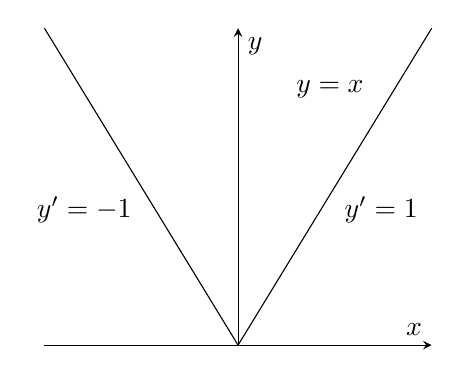
\begin{tikzpicture}
\begin{axis}[clip=false,small,axis lines=middle,xlabel={$x$},ylabel={$y$},xtick={\empty},ytick={\empty}]
\addplot[domain=-4:0]{-x}node[pos=0.5,below left]{$y'=-1$};
\addplot[domain=0:4]{x}node[pos=0.5,below right]{$y'=1$};
\draw(axis cs:1,3)node[above right]{$y=\abs{x}$};
\end{axis}
\end{tikzpicture}
\caption{چونکہ مبدا پر بائیں ہاتھ اور دائیں ہاتھ تفرق مختلف ہیں لہٰذا مبدا پر تفاعل کا تفرق غیر موجود ہے (مثال \حوالہ{مثال_تفرق_مبدا_پر_غیر_موجود})۔}
\label{شکل_مثال_تفرق_مبدا_پر_غیر_موجود}
\end{minipage}
\end{figure}

تفاعل کے دائرہ کار میں کہیں پر بھی تفاعل کے دائیں ہاتھ اور بائیں ہاتھ تفرق  معین ہو سکتے ہیں۔یک طرفہ اور دو طرفہ حد کا تعلق ان تفرق پر بھی قابل اطلاق ہو گا۔  مسئلہ \حوالہ{مسئلہ_حد_یک_طرفہ_بالمقابل_دو_طرفہ_حد} کی بنا کسی نقطے پر تفاعل کا تفرق صرف اور صرف اس صورت موجود ہو گا جب اس نقطے پر تفاعل کے بائیں ہاتھ تفرق اور دائیں ہاتھ تفرق موجود ہوں اور ایک دوسرے کے برابر ہوں۔

\ابتدا{مثال}\شناخت{مثال_تفرق_مبدا_پر_غیر_موجود}
تفاعل \عددی{y=\abs{x}} وقفہ \عددی{(-\infty,0)} اور \عددی{(0,\infty)} پر قابل تفرق ہے لیکن \عددی{x=0} پر اس کا تفرق موجود نہیں ہے۔مبدا کے دائیں جانب
\begin{align*}
\frac{\dif}{\dif x}(\abs{x})=\frac{\dif }{\dif x} (x)=\frac{\dif}{\dif x}(1\cdot x)=1,&& \tfrac{\dif}{\dif x}(mx+b)=m
\end{align*}
ہے جبکہ مبدا کے بائیں جانب
\begin{align*}
\frac{\dif}{\dif x}(\abs{x})=\frac{\dif }{\dif x} (-x)=\frac{\dif}{\dif x} (-1\cdot x)=-1
\end{align*}
ہے (شکل \حوالہ{شکل_مثال_تفرق_مبدا_پر_غیر_موجود})۔چونکہ مبدا پر تفاعل کا دائیں ہاتھ تفرق اور بائیں ہاتھ تفرق ایک جیسے نہیں ہیں لہٰذا مبدا پر تفاعل کا تفرق نہیں پایا جاتا ہے۔

صفر پر \عددی{\abs{x}} کا دائیں ہاتھ تفرق حاصل کرتے ہیں۔
\begin{align*}
\lim_{h\to 0^+}\frac{\abs{0+h}-\abs{0}}{h}&=\lim_{h\to 0^+}\frac{\abs{h}}{h}\quad\quad \text{\RL{اگر \عددی{h>0}  تب \عددی{\abs{h}=h} ہو گا}}\\
&=\lim_{h\to 0^+}\frac{h}{h}=\lim_{h\to 0^+} 1=1
\end{align*}
صفر پر \عددی{\abs{x}} کا بائیں ہاتھ تفرق حاصل کرتے ہیں۔
\begin{align*}
\lim_{h\to 0^-}\frac{\abs{0+h}-\abs{0}}{h}&=\lim_{h\to 0^-}\frac{\abs{h}}{h}\quad\quad \text{\RL{اگر \عددی{h<0}  تب \عددی{\abs{h}=-h} ہو گا}}\\
&=\lim_{h\to 0^-}\frac{-h}{h}=\lim_{h\to 0^-} -1=-1
\end{align*}
\انتہا{مثال}
%==========================

\جزوحصہء{کسی نقطے پر تفاعل کا تفرق کب نہیں پایا جاتا ہے؟}
اگر نقطہ \عددی{N(x_0,f(x_0))} اور اس کے قریب نقطہ \عددی{Q} سے گزرتے ہوئے سیکنٹ کی ڈھلوان، \عددی{Q} کو \عددی{N} کے نزدیک تر کرنے سے تحدیدی قیمت اختیار کرتی ہو  تب تفاعل \عددی{f(x)} نقطہ \عددی{N} پر قابل تفرق ہو گا۔اگر \عددی{Q} کو \عددی{N} کے نزدیک تر کرنے سے سیکنٹ کی ڈھلوان  تحدیدی قیمت اختیار نہ کرتی ہو یا یہ سیکنٹ انتصابی تحدیدی صورت اختیار کرتی ہو، تب اس تفاعل کا \عددی{N} پر تفرق نہیں پایا جائے گا۔ہموار منحنی والے تفاعل کا درج ذیل صورتوں میں نقطہ \عددی{N} پر تفرق نہیں پایا جائے گا۔
\begin{enumerate}[1.]
\item
نوکدار منحنی۔منحنی کی نوک  پر بائیں تفرق اور دائیں تفرق ایک جیسے نہیں ہوتے ہیں (شکل \حوالہ{شکل_تفرق_نا_قابل_نقطے}-ا)۔
\item
راس، جہاں \عددی{NQ} کی تحدیدی ڈھلوان ایک طرف سے \عددی{\infty} اور دوسری طرف سے \عددی{-\infty} ہوتی ہے (شکل \حوالہ{شکل_تفرق_نا_قابل_نقطے}-ب)۔ 
\item
انتصابی مماس، جہاں دونوں اطراف سے تحدیدی \عددی{NQ} کی ڈھلوان \عددی{\infty} یا \عددی{-\infty} ہوتی ہے (شکل \حوالہ{شکل_تفرق_نا_قابل_نقطے}-ج)۔
\item
عدم استمرار (شکل \حوالہ{شکل_تفرق_نا_قابل_نقطے}-د اور شکل \حوالہ{شکل_تفرق_نا_قابل_نقطے}-ہ)۔
\end{enumerate}

\begin{figure}
\centering
\begin{subfigure}{0.5\textwidth}
\centering
\begin{tikzpicture}
\draw[thick](0,0) to [out=45,in=-110]node[pos=0.2,left]{$Q^-$}coordinate[pos=0.2](kA)coordinate[pos=0.4](kB)coordinate[pos=0.6](kC)coordinate[pos=0.8](kD)coordinate[pos=0.95](kE)(1.5,2)node[shift={(-160:0.3)}]{$N$}coordinate(kN) to [out=-20,in=110]node[pos=0.8,left]{$Q^+$}coordinate[pos=0.8](kAA)coordinate[pos=0.6](kBB)coordinate[pos=0.4](kCC)coordinate[pos=0.2](kDD)coordinate[pos=0.05](kEE)(3,0);
\draw[gray,shorten <=-0.5cm, shorten >=-0.5cm] (kN)--(kA);
\draw[gray,shorten <=-0.5cm, shorten >=-1cm] (kN)--(kB);
\draw[gray,shorten <=-0.5cm, shorten >=-1.5cm] (kN)--(kC);
\draw[gray,shorten <=-0.5cm, shorten >=-2cm] (kN)--(kD);
\draw[shorten <=-0.5cm, shorten >=-2.5cm] (kN)--(kE);
%
\draw[gray,shorten <=-0.5cm, shorten >=-0.5cm] (kN)--(kAA);
\draw[gray,shorten <=-0.5cm, shorten >=-1cm] (kN)--(kBB);
\draw[gray,shorten <=-0.5cm, shorten >=-1.5cm] (kN)--(kCC);
\draw[gray,shorten <=-0.5cm, shorten >=-2cm] (kN)--(kDD);
\draw[shorten <=-0.5cm, shorten >=-2.5cm] (kN)--(kEE);
%
\draw(kA)node[circ]{} (kN)node[circ]{} (kAA)node[circ]{};
\end{tikzpicture}
\caption{نوک پر بائیں اور دائیں تفرق ایک دوسرے سے مختلف ہوتے ہیں۔}
\end{subfigure}%
\begin{subfigure}{0.5\textwidth}
\centering
\begin{tikzpicture}
\draw[thick](0,0) to [out=45,in=-90]node[pos=0.2,left]{$Q^-$}coordinate[pos=0.2](kA)coordinate[pos=0.4](kB)coordinate[pos=0.6](kC)coordinate[pos=0.8](kD)coordinate[pos=0.95](kE)(1.5,2)node[shift={(-160:0.3)}]{$N$}coordinate(kN) to [out=-90,in=135]node[pos=0.8,right,yshift=1mm]{$Q^+$}coordinate[pos=0.8](kAA)coordinate[pos=0.6](kBB)coordinate[pos=0.4](kCC)coordinate[pos=0.2](kDD)coordinate[pos=0.05](kEE)(3,0);
\draw[gray,shorten <=-0.5cm, shorten >=-0.5cm] (kN)--(kA);
\draw[gray,shorten <=-0.5cm, shorten >=-0.75cm] (kN)--(kB);
\draw[gray,shorten <=-0.5cm, shorten >=-1.25cm] (kN)--(kC);
\draw[gray,shorten <=-0.5cm, shorten >=-1.5cm] (kN)--(kD);
\draw[shorten <=-0.5cm, shorten >=-2cm] (kN)--(kE);
%
\draw[gray,shorten <=-0.5cm, shorten >=-0.5cm] (kN)--(kAA);
\draw[gray,shorten <=-0.5cm, shorten >=-0.75cm] (kN)--(kBB);
\draw[gray,shorten <=-0.5cm, shorten >=-1.25cm] (kN)--(kCC);
\draw[gray,shorten <=-0.5cm, shorten >=-1.5cm] (kN)--(kDD);
%
\draw(kA)node[circ]{} (kN)node[circ]{} (kAA)node[circ]{};
\end{tikzpicture}
\caption{راس پر ایک طرف سے ڈھلوان $\infty$ جبکہ دوسری طرف سے $-\infty$ ہوتی ہے۔}
\end{subfigure}
\begin{subfigure}{0.5\textwidth}
\centering
\begin{tikzpicture}
\draw[thick](0,0) to [out=-10,in=90]node[pos=0.2,left]{$Q^-$}coordinate[pos=0.2](kA)coordinate[pos=0.4](kB)coordinate[pos=0.6](kC)coordinate[pos=0.8](kD)coordinate[pos=0.95](kE)++(1.5,-1.5)node[shift={(-160:0.3)}]{$N$}coordinate(kN) to [out=-90,in=170]node[pos=0.8,right,yshift=1mm]{$Q^+$}coordinate[pos=0.8](kAA)coordinate[pos=0.6](kBB)coordinate[pos=0.4](kCC)coordinate[pos=0.2](kDD)coordinate[pos=0.05](kEE)++(1.5,-1.5);
\draw[gray,shorten <=-0.5cm, shorten >=-0.5cm] (kN)--(kA);
\draw[gray,shorten <=-0.5cm, shorten >=-0.75cm] (kN)--(kB);
\draw[gray,shorten <=-0.5cm, shorten >=-1cm] (kN)--(kC);
\draw[gray,shorten <=-0.5cm, shorten >=-1.25cm] (kN)--(kD);
%\draw[shorten <=-0.5cm, shorten >=-1.5cm] (kN)--(kE);
\draw[shorten <=-1.5cm](kN)--++(90:1.5);
%
\draw[gray,shorten <=-0.5cm, shorten >=-0.5cm] (kN)--(kAA);
\draw[gray,shorten <=-0.5cm, shorten >=-0.75cm] (kN)--(kBB);
\draw[gray,shorten <=-0.5cm, shorten >=-1cm] (kN)--(kCC);
\draw[gray,shorten <=-0.5cm, shorten >=-1.25cm] (kN)--(kDD);
%\draw[shorten <=-0.5cm, shorten >=-1.5cm] (kN)--(kEE);
%
\draw(kA)node[circ]{} (kN)node[circ]{} (kAA)node[circ]{};
\end{tikzpicture}
\caption{نقطہ $N$ پر مماس انتصابی ہے۔}
\end{subfigure}%
\begin{subfigure}{0.5\textwidth}
\centering
\begin{tikzpicture}
\draw[thick](0,0) to [out=10,in=-135]node[pos=0.2,shift={(135:0.3)}]{$Q^-$}coordinate[pos=0.2](kA)coordinate[pos=0.4](kB)coordinate[pos=0.6](kC)coordinate[pos=0.8](kD)coordinate[pos=1](kE)++(1.5,1) ++(0,1)node[shift={(-160:0.3)}]{$N$}coordinate(kN) to [out=-10,in=135]node[pos=0.8,left]{$Q^+$}coordinate[pos=0.8](kAA)coordinate[pos=0.6](kBB)coordinate[pos=0.4](kCC)coordinate[pos=0.2](kDD)coordinate[pos=0.05](kEE)++(1.5,-1.5);
\draw[gray,shorten <=-0.5cm, shorten >=-0.5cm] (kN)--(kA);
\draw[gray,shorten <=-0.5cm, shorten >=-0.5cm] (kN)--(kB);
\draw[gray,shorten <=-0.5cm, shorten >=-0.5cm] (kN)--(kC);
\draw[gray,shorten <=-0.5cm, shorten >=-0.75cm] (kN)--(kD);
\draw[shorten <=-0.5cm, shorten >=-1cm] (kN)--(kE);
%
\draw[gray,shorten <=-0.5cm, shorten >=-0.5cm] (kN)--(kAA);
\draw[gray,shorten <=-0.5cm, shorten >=-0.75cm] (kN)--(kBB);
\draw[gray,shorten <=-0.5cm, shorten >=-1cm] (kN)--(kCC);
\draw[gray,shorten <=-0.5cm, shorten >=-1.25cm] (kN)--(kDD);
\draw[shorten <=-0.5cm, shorten >=-1.5cm] (kN)--(kEE);
%
\draw(kA)node[circ]{} (kN)node[circ]{} (kAA)node[circ]{} (kE)node[ocirc]{};
\end{tikzpicture}
\caption{عدم استمرار}
\end{subfigure}
\begin{subfigure}{0.5\textwidth}
\centering
\begin{tikzpicture}
\draw[thick](0,0) to [out=-45,in=-180]node[pos=0.2,above]{$Q^-$}coordinate[pos=0.2](kA)coordinate[pos=0.4](kB)coordinate[pos=0.6](kC)coordinate[pos=0.8](kD)coordinate[pos=1](kE)++(1.5,-1)coordinate(kNN) to [out=0,in=135]node[pos=0.8,above right]{$Q^+$}coordinate[pos=0.8](kAA)coordinate[pos=0.6](kBB)coordinate[pos=0.4](kCC)coordinate[pos=0.2](kDD)coordinate[pos=0.05](kEE)++(1.5,-1);
\draw(kNN)++(0,1.5)coordinate(kN)node[right]{$N$};
\draw[gray,shorten <=-0.5cm, shorten >=-0.5cm] (kN)--(kA);
\draw[gray,shorten <=-0.5cm, shorten >=-0.5cm] (kN)--(kB);
\draw[gray,shorten <=-0.5cm, shorten >=-0.5cm] (kN)--(kC);
\draw[gray,shorten <=-0.5cm, shorten >=-0.75cm] (kN)--(kD);
\draw[shorten <=-0.5cm, shorten >=-1cm] (kN)--(kE);
%
\draw[gray,shorten <=-0.5cm, shorten >=-0.5cm] (kN)--(kAA);
\draw[gray,shorten <=-0.5cm, shorten >=-0.75cm] (kN)--(kBB);
\draw[gray,shorten <=-0.5cm, shorten >=-1cm] (kN)--(kCC);
\draw[gray,shorten <=-0.5cm, shorten >=-1.25cm] (kN)--(kDD);
%\draw[shorten <=-0.5cm, shorten >=-1.5cm] (kN)--(kEE);
%
\draw(kA)node[circ]{} (kN)node[circ]{} (kAA)node[circ]{} (kE)node[ocirc]{};
\end{tikzpicture}
\caption{عدم استمرار}
\end{subfigure}%
\caption{ان نقطوں کی پہچان جہاں تفاعل نا قابل تفرق ہو گا۔}
\label{شکل_تفرق_نا_قابل_نقطے}
\end{figure}

\جزوحصہء{قابل تفرق تفاعل استمراری ہوں گے}
جس نقطے پر ایک تفاعل قابل تفرق ہو اس پر یہ تفاعل استمراری ہو گا۔

\ابتدا{مسئلہ}\شناخت{مسئلہ_تفرق_قابل_تفرق_استمراری_ہے}
اگر \عددی{x=c} پر \عددی{f} کا تفرق موجود ہو تب \عددی{x=c} پر \عددی{f} استمراری ہو گا۔
\انتہا{مسئلہ}
%=========================
\ابتدا{ثبوت}
ہم جانتے ہیں کہ \عددی{f'(c)} موجود ہے اور ہم نے دکھانا ہے کہ \عددی{\lim_{x\to c}f(x)=f(c)} یا اس کا مماثل \عددی{\lim_{h\to 0}f(c+h)=f(c)} درست ہیں۔ اگر \عددی{h\ne 0} ہو تب درج ذیل ہو گا۔
\begin{align*}
f(c+h)&=f(c)+(f(c+h)-f(c))\\
&=f(c)+\frac{f(c+h)-f(c)}{h}\cdot h
\end{align*}
اب \عددی{h\to 0} لیں۔ مسئلہ \حوالہ{مسئلہ_حد_قواعد-الف} کے تحت درج ذیل ہو گا۔
\begin{align*}
\lim_{h\to 0}f(c+h)&=\lim_{h\to 0} f(c)+\lim_{h\to 0} \frac{f(c+h)-f(c)}{h}\cdot \lim_{h\to 0}h\\
&=f(c)+f'(c)\cdot 0\\
&=f(c)
\end{align*}
\انتہا{ثبوت}
%===========================

اسی قسم کی دلیل سے ثابت ہوتا ہے کہ اگر \عددی{x=c} پر \عددی{f} کا یک طرفہ (بایاں یا دایاں) تفرق پایا جاتا ہو تب \عددی{x=c} پر \عددی{f} اسی طرف (بائیں یا دائیں) سے استمراری ہو گا۔

\موٹا{انتباہ}\quad مسئلہ \حوالہ{مسئلہ_تفرق_قابل_تفرق_استمراری_ہے} کا الٹ درست نہیں ہے یعنی جس نقطے پر تفاعل استمراری ہو اس پر تفاعل نا قابل تفرق ہو سکتا ہے جیسے ہم نے مثال \حوالہ{مثال_تفرق_مبدا_پر_غیر_موجود} میں دیکھا۔

\موٹا{استمراری تفاعل کی ترسیم کتنی غیر ہموار ہو سکتی ہے؟} ہم نے دیکھا کہ مطلق قیمت تفاعل \عددی{y=\abs{x}} ایک نقطہ پر نا قابل تفرق ہوتا ہے۔یوں ہم استمراری دندان ترسیم (شکل \حوالہ{شکل_تفرق_دندان_ترسیم}) بنا سکتے ہیں جو لا متناہی تعداد کے نقطوں پر نا قابل تفرق ہو گا۔
\begin{figure}
\centering
\begin{minipage}{0.45\textwidth}
\centering
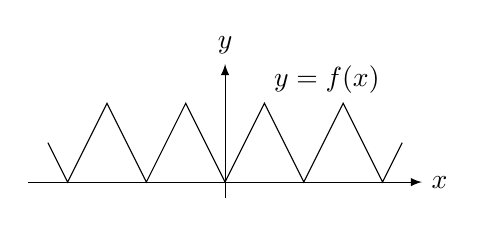
\begin{tikzpicture}[x=0.5cm]
\draw[-latex](-5,0)--(5,0)node[right]{$x$};
\draw[-latex](0,-0.2)--(0,1.5)node[above]{$y$};
\draw(0,0)--++(1,1)node[above right]{$y=f(x)$}--++(1,-1)--++(1,1)--++(1,-1)--++(0.5,0.5);
\draw(0,0)--++(-1,1)--++(-1,-1)--++(-1,1)--++(-1,-1)--++(-0.5,0.5);
\end{tikzpicture}
\caption{دندان ترسیم استمراری لیکن لا متناہی نقطوں پر نا قابل تفرق ہے۔}
\label{شکل_تفرق_دندان_ترسیم}
\end{minipage}\hfill
\begin{minipage}{0.45\textwidth}
\centering
\begin{tikzpicture}
\draw[-latex](-2,0)--(2,0)node[right]{$x$};
\draw[-latex](0,-0.2)--(0,1.5)node[above]{$y$};
\draw[thick](-2,0)--(0,0)node[ocirc]{} (0,1)node[circ]{}--(2,1)node[pos=0.75,above]{$y=\cup(x)$};
\end{tikzpicture}
\caption{اکائی سیڑھی تفاعل متوسط قیمت خاصیت نہیں رکھتا ہے لہٰذا حقیقی خط پر یہ کسی دوسرے تفاعل کا تفرق نہیں ہو سکتا ہے۔}
\label{شکل_تفرق_اکائی_سیڑھی_تفاعل}
\end{minipage}
\end{figure}

\موٹا{کیا استمراری تفاعل ہر نقطے پر نا قابل تفرق ہو سکتا ہے؟} اس کا جواب ہے "جی ہاں" جیسے  \ترچھا{کارل وائشسٹراس}\حاشیہب{جرمن ریاضی دان کارل وائشسٹراس [1815-1897]} نے \سن{1872} میں درج ذیل کلیہ (اور کئی اور) پیش کرتے ہوئے ثابت کیا۔
\begin{align*}
f(x)=\sum_{n=0}^{\infty}\big(\frac{2}{3}\big)^n\cos (9^n\pi x)
\end{align*}
یہ کلیہ \عددی{f} کو  بڑھتی تعدد کے کوسائن تفاعل کے مجموعے کی صورت میں پیش کرتا ہے۔بل کو بل دینے سے ایسا تفاعل حاصل ہوتا ہے جس کا تحدیدی سیکنٹ کسی بھی نقطے پر حاصل کرنا ممکن نہیں ہوتا ہے لہٰذا اس کا مماس کہیں پر بھی نہیں پایا جاتا ہے۔ 

استمراری تفاعل جن کا کسی بھی نقطے پر مماس نہ پایا جاتا ہو \ترچھا{نظریہ ابتری}\فرہنگ{نظریہ!ابتری}\حاشیہب{chaos theory}\فرہنگ{chaos theory} میں کلیدی کردار ادا کرتے ہیں۔ ایسے تفاعل کو متناہی لمبائی مختص کرنا ممکن نہیں ہوتا ہے۔ہم منحنی کی لمبائی اور تفرق کا تعلق پر بعد میں غور کریں گے۔

\جزوحصہء{تفرق کی متوسط قیمت خاصیت}
ضروری نہیں ہے کہ ایک تفاعل کسی دوسرے کا تفرقی تفاعل ہو۔درج ذیل مسئلہ سے اس حقیقت کو اخذ کیا جا سکتا ہے۔

\ابتدا{مسئلہ}\شناخت{مسئلہ_تفرق_متوسط_قیمت_خاصیت}
اگر جس وقفے پر \عددی{f} قابل تفرق ہو اس وقفے میں نقطہ \عددی{a} اور \عددی{b} پائے جاتے ہیں تب  \عددی{f'(a)} اور \عددی{f'(b)} کے بیچ ہر قیمت کا تفرق \عددی{f'} پایا جائے گا۔ 
\انتہا{مسئلہ}
%===========================

مسئلہ \حوالہ{مسئلہ_تفرق_متوسط_قیمت_خاصیت} (جس کا ثبوت ہم پیش نہیں کریں گے)  کہتا ہے کہ کسی وقفے پر ایک تفاعل اس صورت تک کسی دوسرے تفاعل کا تفرق نہیں ہو گا جب تک اس وقفے پر یہ متوسط قیمت خاصیت نہ رکھتا ہو (شکل \حوالہ{شکل_تفرق_اکائی_سیڑھی_تفاعل})۔ ایک تفاعل کب کسی دوسرے تفاعل کا تفرق ہو گا؟ یہ احصاء کی اہم ترین سوالات میں سے ایک ہے جس کا جواب نیوٹن اور لیبنٹز نے دے کر ریاضیات میں انقلاب برپا کیا۔ان کے جواب کو ہم باب میں دیکھیں گے۔

\حصہء{سوالات}
\موٹا{تفرقی تفاعل اور قیمتوں کی تلاش}\\
سوال \حوالہ{سوال_تفرق_قیمت_تلاش_الف} تا سوال \حوالہ{سوال_تفرق_قیمت_تلاش_ب} میں تفرق کی تعریف استعمال کرتے ہوئے دیے گئے تفاعل کے تفرق کی قیمت تلاش کریں۔  

\ابتدا{سوال}\شناخت{سوال_تفرق_قیمت_تلاش_الف}\quad
$f(x)=4-x^2; \quad f'(-3), f'(0), f'(1)$\\
جواب:\quad
$-2x,6,0,-2$
\انتہا{سوال}
%==================
\ابتدا{سوال}
$F(x)=(x-1)^2+1;\quad F'(-1), F'(0), F'(2)$
\انتہا{سوال}
%====================
\ابتدا{سوال}
$g(t)=\tfrac{1}{t^2};\quad g'(-1), g'(2), g'(\sqrt{3})$\\
جواب:\quad
$-\tfrac{2}{t^3},2,-\tfrac{1}{4},-\tfrac{2}{3\sqrt{3}}$
\انتہا{سوال}
%====================
\ابتدا{سوال}
$k(z)=\tfrac{1-z}{2z};\quad k'(-1), k'(1), k'(\sqrt{2})$
\انتہا{سوال}
%====================
\ابتدا{سوال}
$p(\theta)=\sqrt{3\theta};\quad p'(1), p'(3), p'(\tfrac{2}{3})$\\
جواب:\quad
$\tfrac{3}{2\sqrt{3\theta}},\tfrac{3}{2\sqrt{3}},\tfrac{1}{2},\tfrac{3}{2\sqrt{2}}$
\انتہا{سوال}
%====================
\ابتدا{سوال}\شناخت{سوال_تفرق_قیمت_تلاش_ب}\quad
$r(s)=\sqrt{2s+1};\quad r'(0), r'(1), r'(\tfrac{1}{2})$
\انتہا{سوال}
%====================
سوال \حوالہ{سوال_تفرق_درکار_حاصل_الف} تا سوال \حوالہ{سوال_تفرق_درکار_حاصل_ب} میں دیا گیا تفرق حاصل کریں۔

\ابتدا{سوال}\شناخت{سوال_تفرق_درکار_حاصل_الف}
$y=2x^3;\quad \tfrac{\dif y}{\dif x}$\\
جواب:\quad
$6x^2$
\انتہا{سوال}
%========================
\ابتدا{سوال}
$r=\tfrac{s^3}{2}+1;\quad \tfrac{\dif r}{\dif s}$
\انتہا{سوال}
%========================
\ابتدا{سوال}
$s=\tfrac{t}{2t+1};\quad \tfrac{\dif s}{\dif t}$\\
جواب:\quad
$\tfrac{1}{(2t+1)^2}$
\انتہا{سوال}
%========================
\ابتدا{سوال}
$v=t-\tfrac{1}{t};\quad \tfrac{\dif v}{\dif t}$
\انتہا{سوال}
%========================
\ابتدا{سوال}
$p=\tfrac{1}{\sqrt{q+1}};\quad \tfrac{\dif p}{\dif q}$\\
جواب:\quad
 $-\tfrac{1}{2(q+1)\sqrt{q+1}}$
\انتہا{سوال}
%========================
\ابتدا{سوال}\شناخت{سوال_تفرق_درکار_حاصل_ب}
$z=\tfrac{1}{\sqrt{3w-2}};\quad \tfrac{\dif z}{\dif w}$
\انتہا{سوال}
%========================
\موٹا{ڈھلوان اور مماسی خطوط}\\
سوال \حوالہ{سوال_تفرق_ڈھلوان_تلاش_الف} تا سوال \حوالہ{سوال_تفرق_ڈھلوان_تلاش_ب} میں تفاعل کا تفرق حاصل کرتے ہوئے دیے گئے غیر تابع متغیر پر مماس کی ڈھلوان تلاش کریں۔

\ابتدا{سوال}\شناخت{سوال_تفرق_ڈھلوان_تلاش_الف}
$f(x)=x+\tfrac{9}{x};\quad x=-3$\\
جواب:\quad
$1-\tfrac{9}{x^2},0$
\انتہا{سوال}
%=====================
\ابتدا{سوال}
$k(x)=\tfrac{1}{2+x};\quad x=2$
\انتہا{سوال}
%=====================
\ابتدا{سوال}
$s=t^3-t^2;\quad t=-1$\\
جواب:\quad
$3t^2-2t,5$
\انتہا{سوال}
%=====================
\ابتدا{سوال}\شناخت{سوال_تفرق_ڈھلوان_تلاش_ب}
$y=(x+1)^3;\quad x=-2$
\انتہا{سوال}
%=====================
سوال \حوالہ{سوال_تفرق_مماس_مساوات_الف} تا سوال \حوالہ{سوال_تفرق_مماس_مساوات_ب} میں تفاعل کا تفرق حاصل کریں۔ ترسیم پر دیے گئے نقطے پہ تفاعل کے مماس کی مساوات تلاش کریں۔

\ابتدا{سوال}\شناخت{سوال_تفرق_مماس_مساوات_الف}
$f(x)=\tfrac{8}{\sqrt{x-2}};\quad (x,y)=(6,4)$\\
جواب:\quad
$\tfrac{-4}{(x-2)\sqrt{x-2}},y-4=-\tfrac{1}{2}(x-6)$
\انتہا{سوال}
%======================
\ابتدا{سوال}\شناخت{سوال_تفرق_مماس_مساوات_ب}
$g(z)=1+\sqrt{4-z};\quad (z,w)=(3,2)$
\انتہا{سوال}
%======================
سوال \حوالہ{سوال_تفرق_قیمت_نقطے_پر_تلاش_الف} تا سوال \حوالہ{سوال_تفرق_قیمت_نقطے_پر_تلاش_ب} میں تفرق کی قیمت تلاش کریں۔

\ابتدا{سوال}\شناخت{سوال_تفرق_قیمت_نقطے_پر_تلاش_الف}
$\left. \tfrac{\dif s}{\dif t}\right\vert_{t=-1};\quad s=1-3t^2$\\
جواب:\quad
$6$
\انتہا{سوال}
%======================
\ابتدا{سوال}
$\left. \tfrac{\dif y}{\dif x}\right\vert_{x=\sqrt{3}};\quad y=1-\tfrac{1}{x}$
\انتہا{سوال}
%======================
\ابتدا{سوال}
$\left. \tfrac{\dif r}{\dif \theta}\right\vert_{\theta=0};\quad r=\tfrac{2}{\sqrt{4-\theta}}$\\
جواب:\quad
$\tfrac{1}{8}$
\انتہا{سوال}
%======================
\ابتدا{سوال}\شناخت{سوال_تفرق_قیمت_نقطے_پر_تلاش_ب}
$\left. \tfrac{\dif w}{\dif z}\right\vert_{z=4};\quad w=z+\sqrt{z}$
\انتہا{سوال}
%======================
\موٹا{تفرق کے حصول کا متبادل کلیہ}\\
تحدیدی سیکنٹ سے تفرق کا حاصل کلیہ مستعمل نقطوں کی علامتی اظہار پر منحصر ہوتا ہے۔شکل \حوالہ{شکل_تفرق_متبادل_طریقہ} میں سیکنٹ کی ڈھلوان \عددی{\tfrac{f(x)-f(c)}{x-c}} ہے جس کی \عددی{N} پر  تحدیدی قیمت (\عددی{Q} کو \عددی{N} کے نزدیک تر کرتے ہوئے) \عددی{N} پر تفاعل کا تفرق دیتی ہے۔
\begin{align}\label{مساوات_تفرق_متبادل_کلیہ}
f'(c)=\lim_{x\to c} \frac{f(x)-f(c)}{x-c}
\end{align}
%
\begin{figure}
\centering
\begin{tikzpicture}[font=\small,declare function={f(\x)=2-sin(\x);}]
\pgfmathsetmacro{\kS}{70}
\pgfmathsetmacro{\kE}{260}
\pgfmathsetmacro{\kN}{\kS+0.1*(\kE-\kS)}
\pgfmathsetmacro{\kQ}{\kS+0.7*(\kE-\kS)}
\draw(0,0)--(5,0);
\draw[domain=\kS:\kE] plot ({\x*pi/180},{f(\x)})node[above]{$y=f(x)$};
\draw[shorten <=-0.5cm, shorten >=-0.5cm] ({\kN*pi/180},{f(\kN)})node[circ]{}coordinate(kA)node[above,xshift=-2mm,yshift=2mm]{$N(c,f(c))$}--({\kQ*pi/180},{f(\kQ)})node[circ]{}coordinate(kB)node[left,yshift=2mm]{$Q(x,f(x))$};
\draw[dashed](kA)--($(0,0)!(kA)!(5,0)$)node[circ]{}node[below]{$c$}coordinate[pos=0.4](kL);
\path[name path=kR](kB)--($(0,0)!(kB)!(5,0)$);
\path[name path=kH](kA)--++(5,0);
\draw[name intersections={of={kH and kR}}] (kA)--(intersection-1)--(kB);
\draw[dashed] (intersection-1)--($(0,0)!(intersection-1)!(5,0)$)node[circ]{}node[below]{$x$}coordinate(kRB);
\draw[stealth-stealth](kL)--($(intersection-1)!(kL)!(kRB)$)node[pos=0.5,fill=white]{$h=x-c$};
\draw(kB)++(0.3,0)--++(0.3,0)coordinate[pos=0.5](kTop);
\draw(intersection-1)++(0.3,0)--++(0.3,0)coordinate[pos=0.5](kBot);
\draw[stealth-stealth](kTop)--(kBot)node[pos=0.5,right]{$f(x)-f(c)$};
\end{tikzpicture}
\caption{حصول تفرق کا متبادل کلیہ}
\label{شکل_تفرق_متبادل_طریقہ}
\end{figure} 

اس کلیہ کا استعمال چند تفرق کا حصول آسان بناتا ہے۔سوال \حوالہ{سوال_تفرق_متبادل_الف} تا سوال \حوالہ{سوال_تفرق_متبادل_ب} میں اس کلیہ کی مدد سے \عددی{c} پر تفاعل کا تفرق حاصل کریں۔  

\ابتدا{سوال}\شناخت{سوال_تفرق_متبادل_الف}
$f(x)=\tfrac{1}{x+2},\quad c=-1$\\
جواب:\quad
$-1$
\انتہا{سوال}
%=====================
\ابتدا{سوال}
$f(x)=\tfrac{1}{(x-1)^2},\quad c=2$
\انتہا{سوال}
%=====================
\ابتدا{سوال}
$g(t)=\tfrac{t}{t-1},\quad c=3$\\
جواب:\quad
$-\tfrac{1}{4}$
\انتہا{سوال}
%=====================
\ابتدا{سوال}\شناخت{سوال_تفرق_متبادل_ب}
$k(s)=1+\sqrt{s},\quad c=9$
\انتہا{سوال}
%=====================
\موٹا{ترسیمات}
سوال \حوالہ{سوال_شکل_تفرق_اصل_تلاش_الف} تا سوال \حوالہ{سوال_شکل_تفرق_اصل_تلاش_ب} میں دیے گئے تفاعل کا تفرق شکل \حوالہ{شکل_تفرق_اصل_تلاش} میں تلاش کریں۔
\begin{figure}
\centering
\begin{minipage}{1\textwidth}
\begin{subfigure}{0.25\textwidth}
\centering
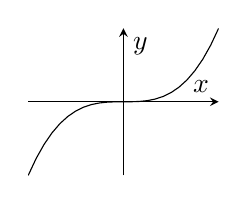
\begin{tikzpicture}[]
\begin{axis}[small,width=4cm,axis lines=middle,xlabel={$x$},ylabel={$y$},xtick={\empty},ytick={\empty}]
\addplot[domain=-2:2]{x^3};
\end{axis}
\end{tikzpicture}
\caption{}
\end{subfigure}%
\begin{subfigure}{0.25\textwidth}
\centering
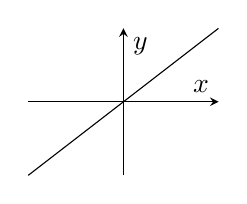
\begin{tikzpicture}[]
\begin{axis}[small,width=4cm,axis lines=middle,xlabel={$x$},ylabel={$y$},xtick={\empty},ytick={\empty}]
\addplot[domain=-2:2]{x};
\end{axis}
\end{tikzpicture}
\caption{}
\end{subfigure}%
\begin{subfigure}{0.25\textwidth}
\centering
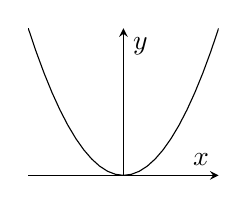
\begin{tikzpicture}[]
\begin{axis}[small,width=4cm,axis lines=middle,xlabel={$x$},ylabel={$y$},xtick={\empty},ytick={\empty}]
\addplot[domain=-2:2]{x^2};
\end{axis}
\end{tikzpicture}
\caption{}
\end{subfigure}%
\begin{subfigure}{0.25\textwidth}
\centering
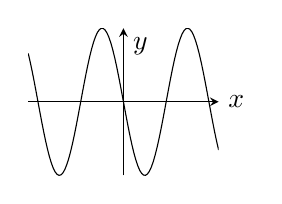
\begin{tikzpicture}[]
\begin{axis}[small,width=4cm,axis lines=middle,xlabel={$x$},ylabel={$y$},xtick={\empty},ytick={\empty},xlabel style={at={(current axis.right of origin)},anchor=west}]
\addplot[domain=-7:7,samples=100]{-sin(deg(x))};
\end{axis}
\end{tikzpicture}
\caption{}
\end{subfigure}
\caption{تفاعل کے تفرق}
\label{شکل_تفرق_اصل_تلاش}
\end{minipage}
\begin{minipage}{1\textwidth}
\begin{subfigure}{0.25\textwidth}
\centering
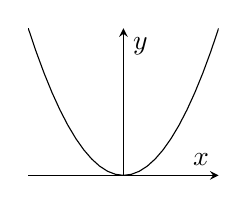
\begin{tikzpicture}[]
\begin{axis}[small,width=4cm,axis lines=middle,xlabel={$x$},ylabel={$y$},xtick={\empty},ytick={\empty}]
\addplot[domain=-2:2]{1/2*x^2};
\end{axis}
\end{tikzpicture}
\caption{}
\end{subfigure}%
\begin{subfigure}{0.25\textwidth}
\centering
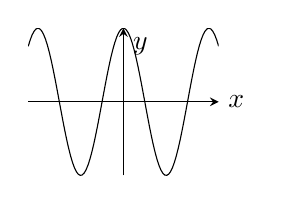
\begin{tikzpicture}[]
\begin{axis}[small,width=4cm,axis lines=middle,xlabel={$x$},ylabel={$y$},xtick={\empty},ytick={\empty},xlabel style={at={(current axis.right of origin)},anchor=west}]
\addplot[domain=-7:7,samples=100]{cos(deg(x))};
\end{axis}
\end{tikzpicture}
\caption{}
\end{subfigure}%
\begin{subfigure}{0.25\textwidth}
\centering
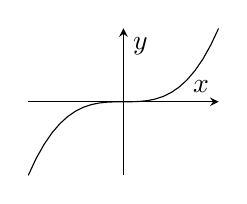
\begin{tikzpicture}[]
\begin{axis}[small,width=4cm,axis lines=middle,xlabel={$x$},ylabel={$y$},xtick={\empty},ytick={\empty}]
\addplot[domain=-2:2]{1/3*x^3};
\end{axis}
\end{tikzpicture}
\caption{}
\end{subfigure}%
\begin{subfigure}{0.25\textwidth}
\centering
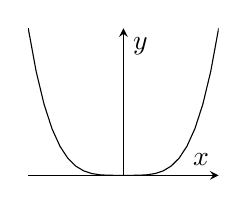
\begin{tikzpicture}[]
\begin{axis}[small,width=4cm,axis lines=middle,xlabel={$x$},ylabel={$y$},xtick={\empty},ytick={\empty}]
\addplot[domain=-1:1]{1/4*x^4};
\end{axis}
\end{tikzpicture}
\caption{}
\end{subfigure}%
\caption{اصل تفاعل}
\label{شکل_تفرق_اصل}
\end{minipage}
\end{figure}

\ابتدا{سوال}\شناخت{سوال_شکل_تفرق_اصل_تلاش_الف}
شکل \حوالہ{شکل_تفرق_اصل}-ا\\
جواب:\quad
شکل \حوالہ{شکل_تفرق_اصل_تلاش}-ب
\انتہا{سوال}
%==============================
\ابتدا{سوال}
شکل \حوالہ{شکل_تفرق_اصل}-ب\\
جواب:\quad
شکل \حوالہ{شکل_تفرق_اصل_تلاش}-د
\انتہا{سوال}
%==============================
\ابتدا{سوال}
شکل \حوالہ{شکل_تفرق_اصل}-ج\\
جواب:\quad
شکل \حوالہ{شکل_تفرق_اصل_تلاش}-ج
\انتہا{سوال}
%==============================
\ابتدا{سوال}\شناخت{سوال_شکل_تفرق_اصل_تلاش_ب}
شکل \حوالہ{شکل_تفرق_اصل}-د\\
جواب:\quad
شکل \حوالہ{شکل_تفرق_اصل_تلاش}-ا
\انتہا{سوال}
%==============================
\ابتدا{سوال}\شناخت{سوال_تفرق_کیا_موجود_الف}
قطعات کو جوڑ کر شکل \حوالہ{شکل_سوال_تفرق_کیا_موجود_الف} حاصل کی گئی ہے۔(ا) وقفہ \عددی{[-4,6]} پر کہاں \عددی{f'} غیر معین ہو گا؟ اپنے جواب کی وجہ پیش کریں۔ (ب) انتصابی محور کو \عددی{y'} کہتے ہوئے \عددی{f'} کو ترسیم کریں۔ترسیم سیڑھی نما ہو گا۔
\begin{figure}
\centering
\begin{minipage}{0.45\textwidth}
\begin{tikzpicture}
\begin{axis}[small,axis lines=middle,xlabel={$x$},ylabel={$y$},xmin=-6,xmax=7.5,ymin=-3,ymax=3,xtick={1,6},ytick={\empty}]
\addplot[] plot coordinates {(-4,0) (0,2) (1,-2) (4,-2) (6,2)};
\draw(axis cs:-4,0)node[circ]{}node[below]{$(-4,0)$}  (axis cs:0,2)node[circ]{}node[left]{$(0,2)$} (axis cs:1,-2)node[circ]{}node[below]{$(1,-2)$}  (axis cs:4,-2)node[circ]{}node[right]{$(4,-2)$} (axis cs:6,2)node[circ]{}node[above]{$(6,2)$} (axis cs:3,1.5)node[]{$y=f(x)$};
\end{axis}
\end{tikzpicture}
\caption{ترسیم برائے سوال \حوالہ{سوال_تفرق_کیا_موجود_الف}}
\label{شکل_سوال_تفرق_کیا_موجود_الف}
\end{minipage}\hfill
\begin{minipage}{0.45\textwidth}
\begin{tikzpicture}
\begin{axis}[small,axis lines=middle,xlabel={$x$},ylabel={$y'$},xmin=-6,xmax=7.5,ymin=-3,ymax=3,xtick={-2,1,3,5},ytick={1}]
\draw[thick](axis cs:-2,-2)node[circ]{}--(axis cs:0,-2)node[ocirc]{}node[right]{$-2$} (axis cs:0,0)node[ocirc]{}--(axis cs:1,0)node[ocirc]{} (axis cs:1,1)node[ocirc]{}--(axis cs:3,1)node[ocirc]{} (axis cs:3,-1)node[ocirc]{}--(axis cs:5,-1)node[circ]{} (axis cs:3,2)node[right]{$y=f'(x)$};
\end{axis}
\end{tikzpicture}
\caption{تفاعل کے تفرق کا ترسیم برائے سوال \حوالہ{سوال_تفرق_سے_اصل_کا_حصول}}
\label{شکل_سوال_تفرق_سے_اصل_کا_حصول}
\end{minipage}
\end{figure}

جواب:\quad
(ا) \عددی{x=0,1,4}؛ (ب) شکل \حوالہ{شکل_سوال_تفرق_کیا_موجود_الف_جواب}
\begin{figure}
\centering
\begin{minipage}{0.45\textwidth}
\centering
\begin{tikzpicture}
\begin{axis}[small,axis lines=middle,xlabel={$x$},ylabel={$y'$},xmin=-5,xmax=7,ymin=-5,ymax=3,ytick={-4,1,2}]
\draw[thick](axis cs:-4,0.5)node[ocirc]{}--(axis cs:0,0.5)node[ocirc]{} (axis cs:0,-4)node[ocirc]{}--(axis cs:1,-4)node[ocirc]{} (axis cs:1,0)node[ocirc]{}--(axis cs:4,0)node[ocirc]{} (axis cs:4,2)node[ocirc]{}--(axis cs:6,2)node[ocirc]{};
\end{axis}
\end{tikzpicture}
\caption{جواب برائے سوال \حوالہ{سوال_تفرق_سے_اصل_کا_حصول}}
\label{شکل_سوال_تفرق_کیا_موجود_الف_جواب}
\end{minipage}
\end{figure}
\انتہا{سوال}
%============================
\ابتدا{سوال}\شناخت{سوال_تفرق_سے_اصل_کا_حصول}\ترچھا{تفاعل کے تفرق سے اصل تفرق کی وصولی}\\
(ا) \quad
درج ذیل طریقے سے تفاعل \عددی{f} ترسیم کو وقفہ \عددی{[-2,5]} پر کریں۔
\begin{enumerate}[1.]
\item
بند قطعات کو جوڑ کر ترسیم حاصل کریں۔
\item
ترسیم کو نقطہ \عددی{(-2,3)} سے شروع کریں۔
\item
تفاعل کا تفرق شکل \حوالہ{شکل_سوال_تفرق_سے_اصل_کا_حصول} میں دکھایا گیا ہے۔
\end{enumerate}
(ب)\quad
نقطہ \عددی{(-2,0)} سے شروع کرتے ہوئے جزو (ا) کا ترسیم دوبارہ حاصل کریں۔
\انتہا{سوال}
%======================
سوال \حوالہ{سوال_تفرق_نا_قابل_الف} تا سوال \حوالہ{سوال_تفرق_نا_قابل_د} میں نقطہ \عددی{N} پر بائیں اور دائیں ہاتھ تفرق کا موازنہ کرتے ہوئے دکھائیں کہ اس نقطے پر تفاعل نا قابل تفرق ہے۔

\ابتدا{سوال}\شناخت{سوال_تفرق_نا_قابل_الف}
تفاعل کو شکل  \حوالہ{شکل_سوال_تفرق_نا_قابل_الف} میں دکھایا گیا ہے۔\\
جواب:\quad
چونکہ \عددی{\lim_{x\to 0^+}f'(x)=1} جبکہ \عددی{\lim_{x\to 0^-}f'(x)=0} ہے لہٰذا \عددی{x=0} پر \عددی{f(x)} نا قابل تفرق ہے۔
 \begin{figure}
\centering
\begin{minipage}{0.25\textwidth}
\centering
\begin{tikzpicture}
\begin{axis}[clip=false,small,width=4cm,axis lines=middle,xlabel={$x$},ylabel={$y$},xtick={\empty},ytick={\empty},ymin=-0.5,font=\footnotesize,ylabel style={at={(current axis.above origin)},anchor=south},xlabel style={at={(current axis.right of origin)},anchor=west}]
\addplot[domain=-1.4142:0]{x^2}node[pos=0.5,fill=white]{$y=x^2$};
\addplot[domain=0:2]{x}node[pos=0.5,fill=white]{$y=x$};
\draw(axis cs:0,0)node[circ]{}node[below right]{$N(0,0)$};
\draw(axis cs:0,2)node[right]{$y=f(x)$};
\end{axis}
\end{tikzpicture}
\caption{}
\label{شکل_سوال_تفرق_نا_قابل_الف}
\end{minipage}\hfill
\begin{minipage}{0.25\textwidth}
\centering
\begin{tikzpicture}
\begin{axis}[clip=false,small,width=4cm,axis lines=middle,xlabel={$x$},ylabel={$y$},xtick={\empty},ytick={\empty},ymin=-0.5,font=\footnotesize,ylabel style={at={(current axis.above origin)},anchor=south},xtick={1,2},ytick={1,3},xmax=3,xlabel style={at={(current axis.right of origin)},anchor=west}]
\addplot[] plot coordinates {(-2,2) (1,2)};
\addplot[domain=1:2]{2*x}node[pos=0.5,right]{$y=2x$};
\draw(axis cs:1,2)node[circ]{}node[below right]{$N(1,2)$};
\draw(axis cs:0,4)node[left]{$y=f(x)$};
\draw(axis cs:-2,2)node[above]{$y=2$};
\end{axis}
\end{tikzpicture}
\caption{}
\label{شکل_سوال_تفرق_نا_قابل_ب}
\end{minipage}\hfill
\begin{minipage}{0.25\textwidth}
\centering
\begin{tikzpicture}
\begin{axis}[clip=false,small,width=4cm,axis lines=middle,xlabel={$x$},ylabel={$y$},xtick={\empty},ytick={\empty},ymin=-0.5,font=\footnotesize,ylabel style={at={(current axis.above origin)},anchor=south},xtick={1},ytick={1},xmax=3,xlabel style={at={(current axis.right of origin)},anchor=west}]
\addplot[domain=0:1]{sqrt(x)}node[pos=0.3,right]{$y=\sqrt{x}$};
\addplot[domain=1:2]{2*x-1}node[pos=0.5,fill=white]{$y=2x-1$};
\draw(axis cs:1,1)node[circ]{}node[right]{$N(1,1)$};
\draw(axis cs:0,3)node[right]{$y=f(x)$};
\end{axis}
\end{tikzpicture}
\caption{}
\label{شکل_سوال_تفرق_نا_قابل_ج}
\end{minipage}\hfill
\begin{minipage}{0.25\textwidth}
\centering
\begin{tikzpicture}
\begin{axis}[clip=false,small,width=4cm,axis lines=middle,xlabel={$x$},ylabel={$y$},xtick={\empty},ytick={\empty},ymin=-0.5,font=\footnotesize,ylabel style={at={(current axis.above origin)},anchor=south},xtick={1},ytick={1},xmax=3,ymax=2,xlabel style={at={(current axis.right of origin)},anchor=west}]
\addplot[domain=-1:1]{x}node[pos=0.15,right]{$y=x$};
\addplot[domain=1:2.5]{1/x}node[pos=0.5,above right]{$y=\tfrac{1}{x}$};
\draw(axis cs:1,1)node[circ]{}node[above]{$N(1,1)$};
\draw(axis cs:0,2)node[right]{$y=f(x)$};
\end{axis}
\end{tikzpicture}
\caption{}
\label{شکل_سوال_تفرق_نا_قابل_د}
\end{minipage}%
\end{figure}
\انتہا{سوال}
%======================
\ابتدا{سوال}\شناخت{سوال_تفرق_نا_قابل_ب}
تفاعل کو شکل  \حوالہ{شکل_سوال_تفرق_نا_قابل_ب} میں دکھایا گیا ہے۔
\انتہا{سوال}
%===========================
\ابتدا{سوال}\شناخت{سوال_تفرق_نا_قابل_ج}
تفاعل کو شکل  \حوالہ{شکل_سوال_تفرق_نا_قابل_ج} میں دکھایا گیا ہے۔\\
جواب:\quad
چونکہ \عددی{\lim_{x\to 1^+}f'(x)=2} جبکہ \عددی{\lim_{x\to 1^-}f'(x)=\tfrac{1}{2}} ہے لہٰذا \عددی{x=1} پر \عددی{f(x)} نا قابل تفرق ہے۔
\انتہا{سوال}
%===========================
\ابتدا{سوال}\شناخت{سوال_تفرق_نا_قابل_د}
تفاعل کو شکل  \حوالہ{شکل_سوال_تفرق_نا_قابل_د} میں دکھایا گیا ہے۔
\انتہا{سوال}
%===========================
سوال \حوالہ{سوال_تفرق_کیا_ہے_الف} تا سوال \حوالہ{سوال_تفرق_کیا_ہے_و} میں بند دائرہ کار \عددی{D} پر تفاعل کا ترسیم دکھایا گیا ہے۔کن نقطوں پر تفاعل (ا) قابل تفرق، (ب) استمراری لیکن نا قابل تفرق، (ج) غیر استمراری اور نا قابل تفرق ہے؟

\ابتدا{سوال}\شناخت{سوال_تفرق_کیا_ہے_الف}
ترسیم شکل \حوالہ{شکل_سوال_تفرق_کیا_ہے_الف} میں دکھایا گیا ہے جبکہ \عددی{D:-3\le x\le 2} ہے۔
\begin{figure}
\centering
\begin{minipage}{0.3\textwidth}
\centering
\begin{tikzpicture}
\begin{axis}[clip=false,small,width=4cm,axis lines=middle,xlabel={$x$},ylabel={$y$},xtick={\empty},ytick={\empty},ymin=-0.5,font=\footnotesize,ylabel style={at={(current axis.above origin)},anchor=south},xtick={-3,-2,1,2},ytick={-2,1,2}, xmin=-3.5, xmax=2.5,ymin=-2.5, ymax=2.5,xlabel style={at={(current axis.right of origin)},anchor=west}]
\draw(axis cs:-3,2)node[circ]{}--(axis cs:2,-2)node[circ]{};
\draw(axis cs:0,1.5)node[right]{$y=f(x)$};
\end{axis}
\end{tikzpicture}
\caption{}
\label{شکل_سوال_تفرق_کیا_ہے_الف}
\end{minipage}\hfill
\begin{minipage}{0.3\textwidth}
\centering
\begin{tikzpicture}
\begin{axis}[clip=false,small,width=4cm,axis lines=middle,xlabel={$x$},ylabel={$y$},xtick={\empty},ytick={\empty},ymin=-0.5,font=\footnotesize,ylabel style={at={(current axis.above origin)},anchor=south},xtick={-3,6},xticklabels={$-2$,$3$},ytick={\empty},xlabel style={at={(current axis.right of origin)},anchor=west},xmin=-4,xmax=7]
\addplot[domain=-3:6,samples=100]{e^(-0.1*x)*sin(deg(x+3))}node[pos=0,circ]{}node[pos=1,circ]{};
\draw(axis cs:0,1)node[right]{$y=f(x)$};
\end{axis}
\end{tikzpicture}
\caption{}
\label{شکل_سوال_تفرق_کیا_ہے_ب}
\end{minipage}\hfill
\begin{minipage}{0.3\textwidth}
\centering
\begin{tikzpicture}
\begin{axis}[clip=false,small,width=4cm,axis lines=middle,xlabel={$x$},ylabel={$y$},xtick={\empty},ytick={\empty},ymin=-0.5,font=\footnotesize,ylabel style={at={(current axis.above origin)},anchor=south},xtick={-3,3},xticklabels={$-3$,$3$},ytick={-3,3},xlabel style={at={(current axis.right of origin)},anchor=west},xmin=-4,xmax=4,ymin=-4,ymax=4]
\draw(axis cs:-3,0) to [out=10,in=-100] node[pos=0,circ]{}node[pos=1,ocirc]{}(axis cs:0,3);
\draw(axis cs:0,-3) to [out=80,in=-170]node[pos=0,ocirc]{}node[pos=1,circ]{} (axis cs:3,0);
\draw(axis cs:0,0)node[circ]{};
\draw(axis cs:0,2)node[right]{$y=f(x)$};
\end{axis}
\end{tikzpicture}
\caption{}
\label{شکل_سوال_تفرق_کیا_ہے_ج}
\end{minipage}
\begin{minipage}{0.3\textwidth}
\centering
\begin{tikzpicture}
\begin{axis}[clip=false,small,width=4cm,axis lines=middle,xlabel={$x$},ylabel={$y$},xtick={\empty},ytick={\empty},ymin=-0.5,font=\footnotesize,ylabel style={at={(current axis.above origin)},anchor=south},xtick={-2,-1,2,3},ytick={1,2,3},xlabel style={at={(current axis.right of origin)},anchor=west},xmin=-2.5,xmax=3.5,ymax=5]
\draw(axis cs:-2,3)--(axis cs:-1,0)node[pos=0,circ]{}--(axis cs:0,3)node[pos=1,ocirc]{};
\addplot[domain=0:3]{3/2.25*(2.25-(x-1.5)^2)}node[pos=0,circ]{}node[pos=1,circ]{};
\draw(axis cs:2,2.667)node[ocirc]{} (axis cs:2,1.5)node[circ]{};
\draw(axis cs:0,4)node[right]{$y=f(x)$};
\end{axis}
\end{tikzpicture}
\caption{}
\label{شکل_سوال_تفرق_کیا_ہے_د}
\end{minipage}\hfill
\begin{minipage}{0.3\textwidth}
\centering
\begin{tikzpicture}
\begin{axis}[clip=false,small,width=4cm,axis lines=middle,xlabel={$x$},ylabel={$y$},xtick={\empty},ytick={\empty},ymin=-0.5,font=\footnotesize,ylabel style={at={(current axis.above origin)},anchor=south},xtick={-1,1,2},ytick={1},xlabel style={at={(current axis.right of origin)},anchor=west},xmin=-1.5,xmax=2.5,ymin=-0.2,ymax=4]
\draw(axis cs:-1,1)node[circ]{} to [out=-20,in=90] (axis cs:0,0) to [out=90,in=-170] (axis cs:2,2)node[circ]{};
\draw(axis cs:0,3)node[right]{$y=f(x)$};
\end{axis}
\end{tikzpicture}
\caption{}
\label{شکل_سوال_تفرق_کیا_ہے_ہ}
\end{minipage}\hfill
\begin{minipage}{0.3\textwidth}
\centering
\begin{tikzpicture}
\begin{axis}[clip=false,small,width=4cm,axis lines=middle,xlabel={$x$},ylabel={$y$},xtick={\empty},ytick={\empty},ymin=-0.5,font=\footnotesize,ylabel style={at={(current axis.above origin)},anchor=south},xtick={-3,-2,-1,1,2,3},xticklabels={,$-2$,$-1$,$1$,$2$,},ytick={2,4},xlabel style={at={(current axis.right of origin)},anchor=west},xmin=-3.5,xmax=3.5,ymin=-1.5,ymax=5]
\addplot[domain=-2:2]{x^2};
\addplot[domain=-2:-3]{8-x^2}node[pos=1,circ]{};
\addplot[domain=2:3]{8-x^2}node[pos=1,circ]{};
\draw(axis cs:0,5)node[right]{$y=f(x)$};
\end{axis}
\end{tikzpicture}
\caption{}
\label{شکل_سوال_تفرق_کیا_ہے_و}
\end{minipage}
\end{figure}

جواب:\quad
(ا) \عددی{-3\le x\le 2} (ب) کوئی نہیں (ج) کوئی نہیں۔
\انتہا{سوال}
%==================
\ابتدا{سوال}\شناخت{سوال_تفرق_کیا_ہے_ب}
ترسیم شکل \حوالہ{شکل_سوال_تفرق_کیا_ہے_ب} میں دکھایا گیا ہے جبکہ \عددی{D:-2\le x\le 3} ہے۔
\انتہا{سوال}
%==================================
\ابتدا{سوال}\شناخت{سوال_تفرق_کیا_ہے_ج}
ترسیم شکل \حوالہ{شکل_سوال_تفرق_کیا_ہے_ج} میں دکھایا گیا ہے جبکہ \عددی{D:-3\le x\le 3} ہے۔\\
جواب:\quad
(ا) \عددی{-3\le x<0, 0<x\le 3} (ب) کوئی نہیں (ج) \عددی{x=0}
\انتہا{سوال}
%==================================
\ابتدا{سوال}\شناخت{سوال_تفرق_کیا_ہے_د}
ترسیم شکل \حوالہ{شکل_سوال_تفرق_کیا_ہے_د} میں دکھایا گیا ہے جبکہ \عددی{D:-2\le x\le 3} ہے۔
\انتہا{سوال}
%==================================
\ابتدا{سوال}\شناخت{سوال_تفرق_کیا_ہے_ہ}
ترسیم شکل \حوالہ{شکل_سوال_تفرق_کیا_ہے_ہ} میں دکھایا گیا ہے جبکہ \عددی{D:-1\le x\le 2} ہے۔\\
جواب:\quad
(ا) \عددی{-1\le x<0, 0<x\le 2} (ب) \عددی{x=0} (ج) کوئی نہیں۔
\انتہا{سوال}
%==================================
\ابتدا{سوال}\شناخت{سوال_تفرق_کیا_ہے_و}
ترسیم شکل \حوالہ{شکل_سوال_تفرق_کیا_ہے_و} میں دکھایا گیا ہے جبکہ \عددی{D:-3\le x\le 3} ہے۔
\انتہا{سوال}
%==================================
سوال \حوالہ{سوال_تفرق_معلومات_تلاش_کریں_الف} تا سوال \حوالہ{سوال_تفرق_معلومات_تلاش_کریں_ب} میں درج ذیل کریں۔
\begin{enumerate}[a.]
\item
تفاعل \عددی{y=f(x)} کا تفرق \عددی{y'=f'(x)} تلاش کریں۔
\item
\عددی{y=f(x)} اور \عددی{y'=f'(x)} کو علیحدہ محدد پر قریب قریب ترسیم کرتے ہوئے درج ذیل کا جواب دیں۔
\item
\عددی{x} کی کن قیمتوں کے لئے  \عددی{y'} کی قیمت  مثبت، منفی اور صفر ہے۔
\item
\عددی{x} بڑھنے سے \عددی{x} کی قیمتوں کے کن وقفوں پر \عددی{y=f(x)} بڑھتا ہے؟ گھٹتا ہے؟ اس کا جزو (ج) کے جوابات کے ساتھ کیا تعلق ہے؟ (اگلے باب میں اس تعلق پر غور کیا جائے گا۔)
\end{enumerate} 

\ابتدا{سوال}\شناخت{سوال_تفرق_معلومات_تلاش_کریں_الف}
$y=-x^2$\\
جواب:\quad
(ا) \عددی{y'=-2x} (ج) \عددی{x<0,x=0,x>0} (د) \عددی{-\infty<x<0,0<x<\infty}
\انتہا{سوال}
%======================
\ابتدا{سوال}
$y=-\tfrac{1}{x}$
\انتہا{سوال}
%======================
\ابتدا{سوال}\شناخت{سوال_تفرق_درکار_پ}
$y=\tfrac{x^3}{3}$\\
جواب:\quad
(ا) \عددی{y'=x^2}، (ب) شکل \حوالہ{شکل_سوال_تفرق_درکار_پ} ، (ج) \عددی{x\ne 0}، \عددی{x=0}، کوئی نہیں،  (د) \عددی{-\infty<x<\infty}، کوئی نہیں۔
\begin{figure}
\centering
\begin{subfigure}{0.5\textwidth}
\centering
\begin{tikzpicture}
\begin{axis}[small,width=4cm,axis lines=middle,xlabel={$x$},ylabel={$y$},xtick={-1,1},ytick={-1,1},xlabel style={at={(current axis.right of origin)},anchor=west},ylabel style={at={(current axis.above origin)},anchor=south},ymax=2]
\addplot[domain=-1.5:1.5]{x^3/3};
\draw(axis cs:0,1.5)node[right]{$y=\tfrac{x^3}{3}$};
\end{axis}
\end{tikzpicture}
\end{subfigure}%
\begin{subfigure}{0.5\textwidth}
\centering
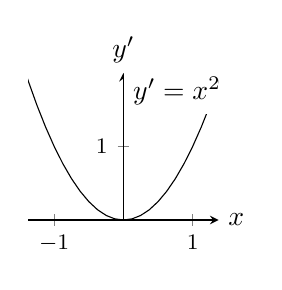
\begin{tikzpicture}
\begin{axis}[small,width=4cm,axis lines=middle,xlabel={$x$},ylabel={$y'$},xtick={-1,1},ytick={1},xlabel style={at={(current axis.right of origin)},anchor=west},ylabel style={at={(current axis.above origin)},anchor=south},ymax=2]
\addplot[domain=-1.5:1.5]{x^2};
\draw(axis cs:0,1.75)node[right,fill=white]{$y'=x^2$};
\end{axis}
\end{tikzpicture}
\end{subfigure}%
\caption{ترسیم برائے شکل \حوالہ{سوال_تفرق_درکار_پ}}
\label{شکل_سوال_تفرق_درکار_پ}
\end{figure}
\انتہا{سوال}
%======================
\ابتدا{سوال}\شناخت{سوال_تفرق_معلومات_تلاش_کریں_ب}
$y=\tfrac{x^4}{4}$
\انتہا{سوال}
%======================
\ابتدا{سوال}
کیا \عددی{y=x^3} کا کبھی منفی ڈھلوان ہو گا؟ اگر ہے تو کہاں ہو گا؟ اپنے جواب کی وجہ پیش کریں۔\\
جواب:\quad
\عددی{y'=3x^2} کبھی بھی منفی نہیں ہو گا۔
\انتہا{سوال}
%======================
\ابتدا{سوال}
کیا \عددی{y=2\sqrt{x}} کا افقی مماس پایا جاتا ہے؟ اگر پایا جاتا ہے تو کہاں پایا جاتا ہے۔ اپنے جواب کی وجہ پیش کریں۔
\انتہا{سوال}
%===========================
\ابتدا{سوال}
کیا قطع مکافی \عددی{y=2x^2-13x+5} کے مماس کا ڈھلوان \عددی{-1} ہو سکتا ہے۔اگر ممکن ہے تب اس مماس کی مساوات حاصل کریں اور وہ نقطہ تلاش کریں جہاں مماس منحنی کو مس کرتا ہے۔ اگر ممکن نہیں ہے تب اپنے جواب کی وجہ پیش کریں۔\\
جواب:\quad
ہاں، \عددی{y+16=-(x-3)} نقطہ \عددی{(3,-16)} پر مماس ہے۔
\انتہا{سوال}
%====================
\ابتدا{سوال}
کیا منحنی \عددی{y=\sqrt{x}} کا کوئی مماس \عددی{x} محور کو \عددی{x=-1} پر قطع کرتا ہے؟ ممکن ہونے کی صورت میں نقطہ مماس اور مماس کی مساوات تلاش کریں جبکہ غیر ممکن ہونے کی صورت میں وجہ پیش کریں۔ 
\انتہا{سوال}
%=======================
\ابتدا{سوال}
کیا \عددی{(-\infty,\infty)} پر قابل تفرق تفاعل کا تفرق \عددی{y=\lfloor x\rfloor} ہو سکتا ہے؟ اپنے جواب کی وجہ پیش کریں۔ \\
جواب:\quad
نہیں، چونکہ تفاعل \عددی{y=\lfloor x\rfloor} متوسط قیمت خاصیت پر پورا نہیں اترتا ہے۔
\انتہا{سوال}
%========================
\ابتدا{سوال}
\عددی{f(x)=\abs{x}} کے تفرق کو ترسیم کرنے کے بعد \عددی{y=\tfrac{\abs{x}-0}{x-0}=\tfrac{\abs{x}}{x}} ترسیم کریں۔ان سے آپ کیا نتیجہ اخذ کر سکتے ہیں؟
\انتہا{سوال}
%========================
\ابتدا{سوال}
یہ جانتے ہوئے کہ \عددی{x=x_0} پر تفاعل \عددی{f(x)} قابل تفرق ہے، آپ \عددی{x=x_0} پر تفاعل \عددی{-f} کی قابل تفرق ہونے کے بارے میں کیا کہہ سکتے ہیں؟ اپنے جواب کی وجہ پیش کریں۔\\
جواب:\quad
ہاں؛ 
$(-f)'(x)=-(f'(x))$
\انتہا{سوال}
%==================
\ابتدا{سوال}
کیا \عددی{t=7} پر \عددی{g(t)} کا قابل تفرق ہونے سے آپ \عددی{t=7} پر \عددی{3g} کے قابل تفرق ہونے کے بارے میں کچھ کہہ سکتے ہیں؟ اپنے جواب کی وجہ پیش کریں۔
\انتہا{سوال}
%======================
\ابتدا{سوال}
فرض کریں کہ \عددی{t} کی تمام قیمتوں کے لئے تفاعل \عددی{g(t)} اور \عددی{h(t)} معین ہیں اور \عددی{g(0)=h(0)=0} ہے۔ کیا \عددی{\lim_{t\to 0}\tfrac{g(t)}{h(t)}} موجود ہو گا؟ اگر حد موجود ہو تب کیا یہ حد ضرور صفر کے برابر ہو گا؟ اپنے جواب کی وجہ پیش کریں۔\\
جواب:\quad
\عددی{g(t)=mt} اور \عددی{h(t)=t} کے لئے \عددی{\lim_{t\to 0}\tfrac{g(t)}{h(t)}=m} ہو گا جو غیر صفر ہو سکتا ہے۔ 
\انتہا{سوال}
%======================
\ابتدا{سوال}
(ا) فرض کریں کہ \عددی{-1\le x\le 1} کے لئے تفاعل \عددی{f(x)} شرط \عددی{\abs{f(x)}\le x^2} کو مطمئن کرتا ہے۔ دکھائیں کہ \عددی{x=0} پر \عددی{f} قابل تفرق ہے اور \عددی{f'(0)} حاصل کریں۔ (ب) دکھائیں کہ \عددی{x=0} پر
\begin{align*}
f(x)=
\begin{cases}
x^2\sin \frac{1}{x},&x\ne 0\\
0,&x=0
\end{cases}
\end{align*}
قابل تفرق ہے اور \عددی{f'(0)} تلاش کریں۔


\انتہا{سوال}
%=========================
\موٹا{کمپیوٹر کا استعمال}

\ابتدا{سوال}
\عددی{0\le x\le 2} کے لئے \عددی{y=\tfrac{1}{2\sqrt{x}}} کو ترسیم کریں۔اس کے اوپر پہلے \عددی{h=1,0.5,0.1} لیتے ہوئے \عددی{y=\tfrac{\sqrt{x+h}-\sqrt{x}}{h}} ترسیم کریں اور بعد میں \عددی{h=-1,-0.5,-0.1} لے کر ترسیم کریں۔سمجھائیں کہ کیا ہو رہا ہے۔
\انتہا{سوال}
%=========================
\ابتدا{سوال}
\عددی{-2\le x\le 2} اور \عددی{0\le y\le 3} لیتے ہوئے \عددی{y=3x^2} ترسیم کریں۔اسی کے اوپر پہلے \عددی{h=2,1,0.2} لیتے ہوئے \عددی{y=\tfrac{(x+h)^3-x^3}{h}} ترسیم کریں اور بعد میں \عددی{h=-2,-1,-0.2} لے کر ترسیم کریں۔ سمجھائیں کیا ہو رہا ہے۔ 
\انتہا{سوال}
%=====================
\ابتدا{سوال}\ترچھا{وائشسٹراس کا نا قابل تفرق تفاعل}
وائشسٹراس تفاعل \عددی{f(x)=\sum_{n=0}^{\infty}()^n\cos(9^n\pi x)} کے پہلے آٹھ ارکان کا مجموعہ درج ذیل ہے۔
\begin{multline*}
g(x)=\cos (\pi x)+\big(\frac{2}{3}\big)^1\cos (9\pi x)+\big(\frac{2}{3}\big)^2\cos (9^2\pi x)\\
+\big(\frac{2}{3}\big)^3\cos (9^3\pi x)+\cdots+\big(\frac{2}{3}\big)^7\cos (9^7\pi x)
\end{multline*}
اس تفاعل کو ترسیم کریں۔ترسیم کی جسامت بڑی کرتے ہوئے دیکھیں کہ یہ کتنی بلدار ہے۔
\انتہا{سوال}
%=====================
سوال \حوالہ{سوال_تفرق_کمپیوٹر_سے_تلاش_الف} تا سوال \حوالہ{سوال_تفرق_کمپیوٹر_سے_تلاش_ب} میں کمپیوٹر استعمال کرتے ہوئے درج ذیل کریں۔
\begin{enumerate}[a.]
\item
\عددی{y=f(x)} ترسیم کرتے ہوئے اس کا رویہ دیکھیں۔
\item
عمومی جسامت قدم \عددی{h} لیتے ہوئے عمومی نقطہ \عددی{x}  پر حاصل تقسیم  \عددی{q} متعارف کریں۔
\item
\عددی{h\to 0} کرتے ہوئے حد لینے سے کون سا کلیہ حاصل ہوتا ہے؟
\item
\عددی{x=x_0} پر کرتے ہوئے تفاعل اور اس نقطے پر مماس ترسیم کریں۔
\item
\عددی{x_0} سے \عددی{x} کی بڑی اور چھوٹی قیمتیں جزو (ج) میں پر کریں۔ کیا کلیہ اور ترسیم ایک جیسا مطلب پیش کرتے ہیں؟
\item
جزو (ج) میں حاصل کیا گیا کلیہ ترسیم کریں۔اس کی قیمتیں منفی، مثبت یا صفر ہونے کا کیا مطلب ہے؟ کیا جزو (ا) کی ترسیم کے ساتھ اس کا کوئی مطلب بنتا ہے؟ اپنے جواب کی وجہ پیش کریں۔
\end{enumerate}

\ابتدا{سوال}\شناخت{سوال_تفرق_کمپیوٹر_سے_تلاش_الف}
$f(x)=x^3+x^2-x,\quad x_0=1$
\انتہا{سوال}
%=====================
\ابتدا{سوال}
$f(x)=x^{\tfrac{1}{3}}+x^{\tfrac{2}{3}},\quad x_0=1$
\انتہا{سوال}
%=====================
\ابتدا{سوال}
$f(x)=\tfrac{4x}{x^2+1},\quad x_0=2$
\انتہا{سوال}
%=====================
\ابتدا{سوال}
$f(x)=\tfrac{x-1}{3x^2+1},\quad x_0=-1$
\انتہا{سوال}
%=====================
\ابتدا{سوال}
$f(x)=\sin 2x,\quad x_0=\tfrac{\pi}{2}$
\انتہا{سوال}
%=====================
\ابتدا{سوال}\شناخت{سوال_تفرق_کمپیوٹر_سے_تلاش_ب}
$f(x)=x^2\cos x,\quad x_0=\tfrac{\pi}{4}$
\انتہا{سوال}
%=====================

\حصہ{قواعد تفرق}
اس حصے میں تفرق کی تعریف استعمال کیے بغیر تفاعل کا تفرق حاصل کرنا سکھایا جائے گا۔

\جزوحصہء{طاقت، مجموعے اور تفریق}
تفرق کا پہلا قاعدہ یہ ہے کہ مستقل کا تفرق صفر کے برابر ہے۔

\ابتدا{قاعدہ}\موٹا{مستقل کا تفرق}\\
اگر \عددی{c} مستقل ہو تب \عددی{\tfrac{\dif}{\dif x} c=0} ہو گا۔
\انتہا{قاعدہ}
%=====================
\ابتدا{مثال}$\frac{\dif}{\dif x} (8)=0,\quad \frac{\dif}{\dif x}\big(-\frac{1}{2}\big)=0,\quad \frac{\dif}{\dif x}(\sqrt{3})=0$
\انتہا{مثال}
%=======================

\ابتدا{ثبوت قاعدہ}
ہم تفرق کی تعریف استعمال کرتے ہوئے \عددی{f(x)=c} کا تفرق حاصل کرتے ہیں (شکل \حوالہ{شکل_تفرق_مستقل_صفر_ہو_گا})۔ہر \عددی{x} پر درج ذیل ہو گا۔
\begin{align*}
f'(x)=\lim_{h\to 0}\frac{f(x+h)-f(x)}{h}=\lim_{h\to 0}\frac{c-c}{h}=\lim_{h\to 0}0=0
\end{align*} 
%
\begin{figure}
\centering
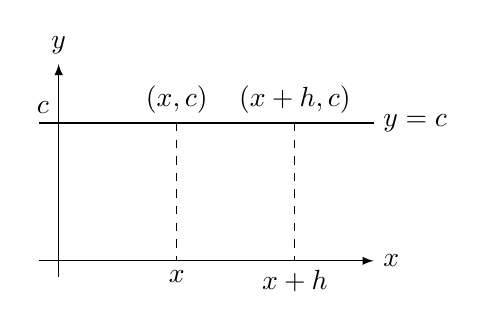
\begin{tikzpicture}
\draw[-latex](-0.25,0)--(4,0)node[right]{$x$};
\draw[-latex](0,-0.2)--(0,2.5)node[above]{$y$};
\draw(-0.25,1.75)--(4,1.75)node[right]{$y=c$};
\draw[dashed](1.5,1.75)node[above]{$(x,c)$}--(1.5,0)node[below]{$x$} (3,1.75)node[above]{$(x+h,c)$}--(3,0)node[below]{$x+h$};
\draw(0,1.75)node[above left]{$c$};
\end{tikzpicture}
\caption{مستقل کا تفرق صفر ہو گا۔}
\label{شکل_تفرق_مستقل_صفر_ہو_گا}
\end{figure}
\انتہا{ثبوت قاعدہ}

اگلا قاعدہ ہمیں \عددی{x^n} کا تفرق دیتا ہے جہاں \عددی{n} مثبت عدد صحیح ہے۔

\ابتدا{قاعدہ}\موٹا{قاعدہ طاقت برائے مثبت عدد صحیح}\\
اگر \عددی{n} مثبت عدد صحیح ہو تب درج ذیل ہو گا۔
\begin{align*}
\frac{\dif}{\dif x} x^n=nx^{n-1}
\end{align*}
\انتہا{قاعدہ}
%=========================

قاعدہ طاقت استعمال کرتے ہوئے ہم  طاقت \عددی{n} سے \عددی{1} منفی کرتے ہوئے جواب کو \عددی{n} سے ضرب دیتے ہیں۔

\ابتدا{مثال}
\begin{align*}
\begin{array}{c|c|c|c|c|c}
f&x&x^2&x^3&x^4&\cdots\\
\hline
f'&1&2x&3x^2&4x^3&\cdots
\end{array}
\end{align*}
\انتہا{مثال}
%=======================
\ابتدا{ثبوت قاعدہ}
اگر \عددی{f(x)=x^n} ہو تب \عددی{f(x+h)=(x+h)^n} ہو گا۔چونکہ \عددی{n} مثبت عدد صحیح ہے ہم درج ذیل حقیقت 
\begin{align*}
a^n-b^n=(a-b)(a^{n-1+a^{n-2}b}+\cdots+ab^{n-2}+b^{n-1})
\end{align*}
استعمال کرتے ہوئے تفریقی حاصل تقسیم کی سادہ صورت حاصل کرتے ہیں۔ہم \عددی{a=x+h} اور \عددی{b=x} لیتے ہیں۔یوں \عددی{h=a-b} ہو گا۔اس طرح 
\begin{align*}
\frac{f(x+h)-f(x)}{h}&=\frac{(x+h)^n-x^n}{h}\\
&=\frac{(h)[(x+h)^{n-1}+(x+h)^{n-2}x+\cdots+(x+h)x^{n-2}+x^{n-1}]}{h}\\
&=(x+h)^{n-1}+(x+h)^{n-2}x+\cdots+(x+h)x^{n-2}+x^{n-1}
\end{align*}
لکھا جا سکتا ہے جو \عددی{n} ارکان پر مشتمل ہے اور  \عددی{h\to 0} کرتے ہوئے ہر رکن کا  حد \عددی{x^{n-1}} ہے۔یوں درج ذیل  نتیجہ حاصل ہوتا ہے۔ 
\begin{align*}
\frac{\dif}{\dif x}x^n=\lim_{h\to 0}\frac{f(x+h)-f(x)}{h}=nx^{n-1}
\end{align*}
\انتہا{ثبوت قاعدہ}
%=======================
اگلا قاعدہ کہتا ہے کہ قابل تفرق تفاعل کو مستقل سے ضرب دینے سے حاصل تفاعل کا تفرق بھی اس مستقل سے ضرب ہو گا۔

\ابتدا{قاعدہ}\شناخت{قاعدہ_تفرق_مضرب_مستقل}\موٹا{قاعدہ مستقل مضرب}\\
اگر \عددی{u} متغیر \عددی{x} کا قابل تفرق تفاعل ہو اور \عددی{c} ایک مستقل ہو تب درج ذیل ہو گا۔
\begin{align*}
\frac{\dif}{\dif x} (cu)=c\frac{\dif u}{\dif x}
\end{align*}
\انتہا{قاعدہ}
%====================

بالخصوص مثبت عدد صحیح \عددی{n} کی صورت میں درج ذیل ہو گا۔
\begin{align*}
\frac{\dif}{\dif x} (cx^n)=cnx^{n-1}
\end{align*}

\ابتدا{مثال}\شناخت{مثال_تفرق_ڈھلوان_اور_مستقل}
تفرقی کلیہ \عددی{\tfrac{\dif}{\dif x}(3x^2)=3\cdot 2x=6x} کہتی ہے کہ \عددی{y} محور کو \عددی{3} سے ضرب دیتے ہوئے ترسیم \عددی{y=x^2} کی پیمائش تبدیل کرنے سے ہر نقطے کی ڈھلوان \عددی{3} سے ضرب ہو گی (شکل \حوالہ{شکل_مثال_تفرق_ڈھلوان_اور_مستقل})۔
\begin{figure}
\centering
\begin{tikzpicture}
\begin{axis}[clip=false,small,axis lines=middle,xlabel={$x$},ylabel={$y$},xtick={1,2},ytick={1,2,3}]
\addplot[domain=-0.25:2]{x^2}node[above,xshift={2mm}]{$y=x^2$};
\addplot[domain=-0.25:1.25]{3*x^2}node[left]{$y=3x^2$};
\draw[dashed](axis cs:1,0)--(axis cs:1,3)node[left]{$(1,3)$};
\draw[dashed](axis cs:1,1)node[circ]{}node[right]{$(1,1)$} (axis cs:1,3)node[circ]{};
\draw[shorten <=-1cm](axis cs:1,1)--(axis cs:1.5,2)node[right]{$m=2$};
\draw[shorten <=-1cm](axis cs:1,3)--(axis cs:1.2,4.2)node[right]{$m=6$};
\end{axis}
\end{tikzpicture}
\caption{ترسیم برائے مثال \حوالہ{مثال_تفرق_ڈھلوان_اور_مستقل}}
\label{شکل_مثال_تفرق_ڈھلوان_اور_مستقل}
\end{figure}
\انتہا{مثال}
%======================
\ابتدا{مثال}
قابل تفرق تفاعل کے منفی کا تفرق اس تفاعل کے تفرق کا منفی ہو گا۔قاعدہ \حوالہ{قاعدہ_تفرق_مضرب_مستقل} میں \عددی{c=-1} لیتے ہوئے درج ذیل ملتا ہے۔
\begin{align*}
\frac{\dif}{\dif x}(-u)=\frac{\dif}{\dif x}(-1\cdot u)=-1\cdot \frac{\dif}{\dif x}(u)=-\frac{\dif u}{\dif x}
\end{align*}
\انتہا{مثال}
%======================

\ابتدا{ثبوت قاعدہ} (قاعدہ \حوالہ{قاعدہ_تفرق_مضرب_مستقل})
\begin{align*}
\frac{\dif}{\dif x} cu&=\lim_{h\to 0}\frac{cu(x+h)-cu(x)}{h}&&\text{\RL{\عددی{f(x)=cu(x)} کے تفرق کی تعریف}}\\
&=c\lim_{h\to 0}\frac{u(x+h)-u(x)}{h} && \text{\RL{تحدیدی خاصیت}}\\
&=c\frac{\dif u}{\dif x}&&\text{\RL{\عددی{u} قابل تفرق ہے}}
\end{align*}
\انتہا{ثبوت قاعدہ}

اگلا قاعدہ کہتا ہے کہ دو قابل تفرق تفاعل کے مجموعے کا تفرق ان کے انفرادی تفرق کا مجموعہ ہو گا۔

\ابتدا{قاعدہ}\شناخت{قاعدہ_تفرق_مجموعہ}\موٹا{قاعدہ مجموعہ}\\
اگر \عددی{u} اور \عددی{v} متغیر \عددی{x} کے قابل تفرق تفاعل ہوں تب ان کا مجموعہ \عددی{u+v} ہر اس نقطے پر قابل تفرق ہو گا جہاں \عددی{u} اور \عددی{v} دونوں قابل تفرق ہوں۔ایسے نقطے پر درج ذیل ہو گا۔
\begin{align*}
\frac{\dif}{\dif x} (u+v)=\frac{\dif u}{\dif x}+\frac{\dif v}{\dif x}
\end{align*}
\انتہا{قاعدہ}
%================================

قاعدہ مجموعہ اور قاعدہ مستقل مضرب کو ملا کر مساوی \اصطلاح{تفریقی قاعدہ} حاصل ہو گا جس کے تحت دو قابل تفرق تفاعل کے حاصل تفریق کا تفرق ان کے تفرق کا تفریق ہو گا:
\begin{align*}
\frac{\dif}{\dif x} (u-v)=\frac{\dif}{\dif x}[u+(-1)v]=\frac{\dif u}{\dif x}+(-1)\frac{\dif v}{\dif x}=\frac{\dif u}{\dif x}-\frac{\dif v}{\dif x}
\end{align*} 

قاعدہ مجموعہ کو وسعت دے کر دو  سے زیادہ تفاعل کے لئے بھی استعمال کیا جا سکتا ہے بس اتنا ضروری ہے کہ مجموعہ میں ارکان کی تعداد متناہی ہو۔اگر \عددی{u_1,u_2,\cdots,u_n} متغیر \عددی{x} کے قابل تفرق تفاعل ہوں تب \عددی{u_1+u_2+\cdots+u_n} بھی قابل تفرق ہو گا اور اس کا تفرق درج ذیل ہو گا۔
\begin{align*}
\frac{\dif}{\dif x}(u_1+u_2+\cdots+u_n)=\frac{\dif u_1}{\dif x}+\frac{\dif u_2}{\dif x}+\cdots+\frac{\dif u_n}{\dif x}
\end{align*}

\ابتدا{مثال}
\begin{gather*}
\begin{aligned}[t]
\text{(ا)}\quad y&=x^4+12x\\
\frac{\dif y}{\dif x}&=\frac{\dif}{\dif x}(x^4)+\frac{\dif}{\dif x}(12x)\\
&=4x^3+12
\end{aligned}
\quad
\begin{aligned}[t]
\text{(ب)}\quad y&=x^3+\frac{4}{3}x^2-5x+1\\
\frac{\dif y}{\dif x}&=\frac{\dif}{\dif x}x^3+\frac{\dif}{\dif x}\big(\frac{4}{3}x^2\big)-\frac{\dif}{\dif x}(5x)+\frac{\dif}{\dif x}(1)\\
&=3x^2+\frac{4}{3}\cdot 2x-5+0\\
&=3x^2+\frac{8}{3}x-5
\end{aligned}
\end{gather*}
\انتہا{مثال}
%======================
آپ نے اس مثال میں دیکھا کہ کسی بھی کثیر رکنی کا جزو در جزو تفرق لیا جا سکتا ہے۔ 

\ابتدا{ثبوت قاعدہ} (قاعدہ \حوالہ{قاعدہ_تفرق_مجموعہ})
ہم تفرق کی تعریف کو \عددی{f(x)=u(x)+v(x)} پر لاگو کرتے ہیں۔
\begin{align*}
\frac{\dif}{\dif x}[u(x)+v(x)]&=\lim_{h\to 0}\frac{[u(x+h)+v(x+h)]-[u(x)+v(x)]}{h}\\
&=\lim_{h\to 0}\left[ \frac{u(x+h)-u(x)}{h}+\frac{v(x+h)-v(x)}{h}\right]\\
&=\lim_{h\to 0}\frac{u(x+h)-u(x)}{h}+\lim_{h\to 0}\frac{v(x+h)-v(x)}{h}\\
&=\frac{\dif u}{\dif x}+\frac{\dif v}{\dif x}
\end{align*}
\انتہا{ثبوت قاعدہ}
%==========================

\موٹا{دو سے زیادہ تفاعل کے مجموعہ کے لئے ثبوت}\\
ہم درج ذیل فقرے کو \اصطلاح{ریاضی ماخوذ}\حاشیہب{mathematical induction} کی مدد سے ثابت کرتے ہیں۔
\begin{align}\label{مساوات_تفرق_مجموعہ_الف}
\frac{\dif}{\dif x}(u_1+u_2+\cdots+u_n)=\frac{\dif u_1}{\dif x}+\frac{\dif u_2}{\dif x}+\cdots+\frac{\dif u_n}{\dif x}
\end{align}
جیسا اوپر ثابت کیا گیا درج بالا فقرہ \عددی{n=2} کے لئے درست ہے۔یہ ریاضی ماخوذ کا پہلا قدم ہے۔

دوسرے قدم میں ہم نے ثابت کرنا ہو گا کہ اگر یہ فقرہ کسی بھی مثبت عدد صحیح \عددی{n=k} (جہاں \عددی{k\ge n_0=2} ہے)  کے لئے درست ہے تب یہ \عددی{n=k+1} کے لئے بھی درست ہو گا۔ فرض کریں کہ
\begin{align*}
\frac{\dif}{\dif x}(u_1+u_2+\cdots+u_k)=\frac{\dif u_1}{\dif x}+\frac{\dif u_2}{\dif x}+\cdots+\frac{\dif u_k}{\dif x}
\end{align*}
ہے تب درج ذیل ہو گا۔
\begin{align*}
&\frac{\dif}{\dif x}(\underbrace{u_1+u_2+\cdots+u_k}_{\text{\RL{اس مجموعہ کو \عددی{u} کہیں}}}+\underbrace{u_{k+1}}_{\text{\RL{اس کو \عددی{v} کہیں}}})\\
&=\frac{\dif}{\dif x}(u_1+u_2+\cdots+u_k)+\frac{\dif u_{k+1}}{\dif x}\\
&=\frac{\dif u_1}{\dif x}+\frac{\dif u_2}{\dif x}+\cdots+\frac{\dif u_k}{\dif x}+\frac{\dif u_{k+1}}{\dif x}
\end{align*}
اس قدم کی تکمیل  ہر عدد صحیح \عددی{n\ge 2} کے لئے  قاعدہ \حوالہ{قاعدہ_تفرق_مجموعہ} کی درستگی کی تصدیق کرتا ہے۔

%=====================
\ابتدا{مثال}\شناخت{مثال_تفرق_ٹیڑی_منحنی}
کیا منحنی \عددی{y=x^4-2x^2+2} کا افقی مماس پایا جاتا ہے؟ اگر پایا جاتا ہے تب کہاں پایا جاتا ہے؟\\
حل:\quad افقی مماس وہاں ہو گا جہاں \عددی{\tfrac{\dif y}{\dif x}} صفر کے برابر ہو۔ان نقطوں کو حاصل کرنے کے لئے ہم \عددی{\tfrac{\dif y}{\dif x}} معلوم کرتے ہیں
\begin{align*}
\frac{\dif y}{\dif x}=\frac{\dif}{\dif x}(x^4-2x^2+2)=4x^3-4x
\end{align*}
اور اس کے بعد مساوات \عددی{\tfrac{\dif y}{\dif x}=0} کو \عددی{x} کے لئے حل کرتے ہیں۔
\begin{align*}
4x^3-4x&=0\\
4x(x^2-1)&=0\\
x&=0,1,-1
\end{align*}
منحنی \عددی{y=x^4-2x^2+2} کا افقی مماس \عددی{x=0,1,-1} پر پایا جاتا ہے جہاں منحنی کے مطابقتی نقطے \عددی{(-1,1)}، \عددی{(1,1)}، \عددی{(0,2)} ہیں (شکل \حوالہ{شکل_مثال_تفرق_ٹیڑی_منحنی})۔
\begin{figure}
\centering
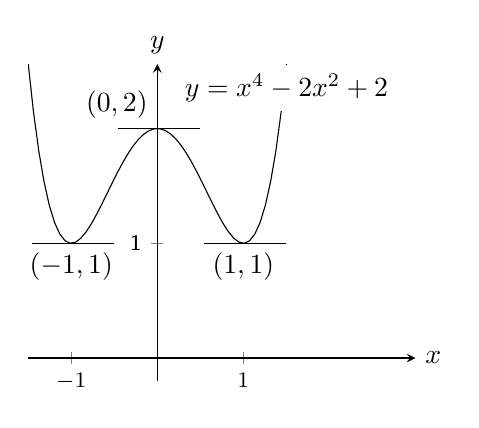
\begin{tikzpicture}
\begin{axis}[small,axis lines=middle,xlabel={$x$},ylabel={$y$},xtick={-1,1},ytick={1,1},ymin=-0.2,xmax=3,xlabel style={at={(current axis.right of origin)},anchor={west}},ylabel style={at={(current axis.above origin)},anchor=south}]
\addplot[domain=-1.5:1.5,samples=50]{x^4-2*x^2+2}node[below,fill=white]{$y=x^4-2x^2+2$};
\draw[shorten <=-0.5cm](axis cs:-1,1)--(axis cs:-0.5,1);
\draw[shorten <=-0.5cm](axis cs:1,1)--(axis cs:1.5,1);
\draw[shorten <=-0.5cm](axis cs:0,2)--(axis cs:0.5,2);
\draw(axis cs:-1,1)node[below]{$(-1,1)$} (axis cs:1,1)node[below]{$(1,1)$} (axis cs:0,2)node[above left]{$(0,2)$};
\end{axis}
\end{tikzpicture}
\caption{افقی مماس (مثال \حوالہ{مثال_تفرق_ٹیڑی_منحنی})}
\label{شکل_مثال_تفرق_ٹیڑی_منحنی}
\end{figure}
\انتہا{مثال}
%=====================
\جزوحصہء{حاصل ضرب اور حاصل تقسیم}
اگرچہ دو تفاعل کے مجموعہ کا تفرق ان تفاعل کے تفرق کا مجموعہ ہے، دو تفاعل کے حاصل ضرب کا تفرق ان تفاعل کے تفرق کا حاصل ضرب \ترچھا{نہیں} ہو گا۔مثال کے طور پر
\begin{align*}
\text{\RL{ہو گا۔}}\quad \frac{\dif}{\dif x}(x)\cdot \frac{\dif}{\dif x}(x)=1\cdot 1=1\quad\text{\RL{ہے جبکہ}}\quad \frac{\dif}{\dif x}(x\cdot x)=\frac{\dif}{\dif x}(x^2)=2x
\end{align*}
دو تفاعل کے حاصل ضرب کا تفرق دو حاصل ضرب کا مجموعہ ہو گا۔

\ابتدا{قاعدہ}\موٹا{قاعدہ حاصل ضرب}\\
اگر \عددی{u} اور \عددی{v} متغیر \عددی{x} کے قابل تفرق تفاعل ہوں تب ان کا حاصل ضرب \عددی{uv} بھی \عددی{x} کا قابل تفرق تفاعل ہو گا جس کا تفرق درج ذیل ہو گا۔
\begin{align*}
\frac{\dif}{\dif x}(uv)=u\frac{\dif v}{\dif x}+v\frac{\dif u}{\dif x}
\end{align*}
\انتہا{قاعدہ}
%========================
حاصل ضرب \عددی{uv} کا تفرق \عددی{u} ضرب \عددی{v} کا تفرق جمع \عددی{v} ضرب \عددی{u} کا تفرق ہو گا۔اس کو \عددی{(uv)'=uv'+vu'} بھی لکھا جا سکتا ہے۔

\ابتدا{ثبوت قاعدہ}
تفرق کی تعریف کے تحت
\begin{align*}
\frac{\dif}{\dif x}(uv)=\lim_{h\to 0}\frac{u(x+h)v(x+h)-u(x)v(x)}{h}
\end{align*}
ہو گا جس کو \عددی{u} اور \عددی{v} کے تفریقی حاصل تقسیم کی صورت میں لکھنے کی خاطر ہم شمار کنندہ میں \عددی{u(x+h)v(x)} جمع اور منفی کرتے ہیں۔
\begin{align*}
\frac{\dif}{\dif x}(uv)&=\lim_{h\to 0}\frac{u(x+h)v(x+h)-u(x+h)v(x)+u(x+h)v(x)-u(x)v(x)}{h}\\
&=\lim_{h\to 0}\left[u(x+h)\frac{v(x+h)-v(x)}{h}+v(x)\frac{u(x+h)-u(x)}{h} \right]\\
&=\lim_{h\to 0} u(x+h)\cdot \lim_{h\to 0}\frac{v(x+h)-v(x)}{h}+v(x)\cdot\lim_{h\to 0}\frac{u(x+h)-u(x)}{h}
\end{align*}
چونکہ \عددی{x} پر \عددی{u} قابل تفرق ہے لہٰذا \عددی{h\to 0} کرنے سے \عددی{u(x+h)\to u(x)} ہو گا۔ دو کسر کی تحدیدی قیمتیں \عددی{x} پر  \عددی{\tfrac{\dif v}{\dif x}} اور \عددی{\tfrac{\dif u}{\dif x}} ہیں۔مختصراً درج ذیل ملتا ہے۔
\begin{align*}
\frac{\dif}{\dif x}(uv)=u\frac{\dif v}{\dif x}+v\frac{\dif u}{\dif x}
\end{align*}
\انتہا{ثبوت قاعدہ}
%============================
\موٹا{قاعدہ حاصل ضرب کی تصور کشی}\\
اگر \عددی{u(x)} اور \عددی{v(x)} مثبت ہوں اور \عددی{x} بڑھنے سے بڑھتے ہوں تب  \عددی{h>0} کی صورت میں شکل \حوالہ{شکل_تفرق_قاعدہ_ضرب_تصور_کشی} حاصل ہو گا۔\عددی{u(x)} اور \عددی{v(x)} بڑھنے سے رقبہ میں اضافہ
\begin{align*}
u(x+h)v(x+h)-u(x)v(x)=u(x+h)\Delta v+v(x+h)\Delta u-\Delta u\Delta v
\end{align*}
ہو گا جس کو ہلکا سیاہ رنگ دیا گیا ہے۔اس مساوات کے دونوں اطراف کو \عددی{h} سے تقسیم  کرنے سے
\begin{align*}
\frac{u(x+h)v(x+h)-u(x)v(x)}{h}&=u(x+h)\frac{\Delta v}{h}+v(x+h)\frac{\Delta u}{h}-\Delta u\frac{\Delta v}{h}
\end{align*}
حاصل ہو گا۔ اب \عددی{h\to 0^+}  کرنے سے \عددی{\Delta u\cdot \tfrac{\Delta v}{h}\to 0\cdot\tfrac{\dif v}{\dif x}=0} ہو گا لہٰذا درج ذیل باقی رہ جاتا ہے۔
\begin{align*}
\frac{\dif}{\dif x}(uv)=u\frac{\dif v}{\dif x}+v\frac{\dif u}{\dif x}
\end{align*} 
%
\begin{figure}
\centering
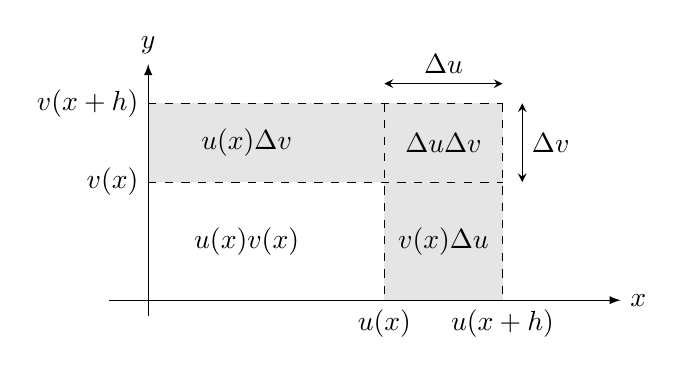
\begin{tikzpicture}
\fill[fill=gray!20](0,0) rectangle(4.5,2.5);
\fill[fill=white](0,0) rectangle(3,1.5);
\draw[-latex](-0.5,0)--(6,0)node[right]{$x$};
\draw[-latex](0,-0.2)--(0,3)node[above]{$y$};
\draw[dashed](0,2.5)node[left]{$v(x+h)$}--(4.5,2.5);
\draw[dashed](0,1.5)node[left]{$v(x)$}--(4.5,1.5);
\draw[dashed] (3,2.5)--(3,0)node[below]{$u(x)$};
\draw[dashed](4.5,2.5)--(4.5,0)node[below]{$u(x+h)$}; 
\draw(1.25,0.75)node[]{$u(x)v(x)$};
\draw(3.75,0.75)node[]{$v(x)\Delta u$};
\draw(1.25,2)node[]{$u(x)\Delta v$};
\draw(3.75,2)node[]{$\Delta u\Delta v$};
\draw[stealth-stealth] (3,2.75)--(4.5,2.75)node[pos=0.5,above]{$\Delta u$};
\draw[stealth-stealth] (4.75,2.5)--(4.75,1.5)node[pos=0.5,right]{$\Delta v$};
\end{tikzpicture}
\caption{قاعدہ حاصل ضرب کی تصور کشی۔}
\label{شکل_تفرق_قاعدہ_ضرب_تصور_کشی}
\end{figure}

%=======================
\ابتدا{مثال}\شناخت{مثال_تفرق_قاعدہ_حاصل_ضرب}
تفاعل \عددی{y=(x^2+1)(x^3+3)} کا تفرق تلاش کریں۔\\
حل:\quad
قاعدہ حاصل ضرب میں \عددی{u=x^2+1} اور \عددی{v=x^3+3} لیتے ہوئے درج ذیل ملتا ہے۔
\begin{align*}
\frac{\dif}{\dif x}[(x^2+1)(x^3+3)]&=(x^2+1)(3x^2)+(x^3+3)(2x)\\
&=3x^4+3x^2+2x^4+6x\\
&=5x^4+3x^2+6x
\end{align*}
\انتہا{مثال}
%=============================
 
اس مثال میں  قوسین کھول کر تفرق لینا غالباً زیادہ بہتر ہوتا۔ایسا کرنے سے
\begin{align*}
y&=(x^2+1)(x^3+3)=x^5+x^3+3x^2+3\\
\frac{\dif y}{\dif x}&=5x^4+3x^2+6x
\end{align*}
ملتا ہے جو مثال \حوالہ{مثال_تفرق_قاعدہ_حاصل_ضرب} میں حاصل جواب کی تصدیق کرتا ہے۔

بعض اوقات آپ دیکھیں گے کہ قاعدہ حاصل ضرب استعمال کرنا ضروری ہو گا یا نسبتاً زیادہ آسان ہو گا۔درج ذیل مثال میں ہمارے پاس صرف اعدادی قیمتیں ہیں جن سے ہمیں جواب حاصل کرنا ہے۔

\ابتدا{مثال}
فرض کریں کہ \عددی{y=uv} تفاعل \عددی{u} اور \عددی{v} کا حاصل ضرب ہے۔درج ذیل استعمال کرتے ہوئے \عددی{y'(2)} تلاش کریں۔
\begin{align*}
u(2)=3,\quad u'(2)=-4,\quad v(2)=1,\quad v'(2)=2
\end{align*}
حل:\quad
قاعدہ حاصل ضرب کی درج ذیل صورت
\begin{align*}
y'=(uv)'=uv'+vu'
\end{align*}
استعمال کرتے ہیں۔
\begin{align*}
y'(2)&=u(2)v'(2)+v(2)u'(2)\\
&=(3)(2)+(1)(-4)=6-4=2
\end{align*}
\انتہا{مثال}
%============================

\جزوحصہء{حاصل تقسیم}
جیسا تفاعل کے حاصل ضرب کا تفرق ان کے تفرق کا حاصل ضرب نہیں تھا اسی طرح تفاعل کے حاصل تقسیم کا تفرق ان کے تفرق کا حاصل تقسیم نہیں ہو گا۔درج ذیل قاعدہ اس کا حل دیتا ہے۔

\ابتدا{قاعدہ}\موٹا{قاعدہ حاصل تقسیم}\\
اگر \عددی{u(x)} اور \عددی{v()} متغیر \عددی{x} کے قابل تفرق تفاعل ہوں تب ان کا حاصل تقسیم \عددی{\tfrac{u}{v}} بھی \عددی{x} کا قابل تفرق تفاعل ہو گا اور یہ تفرق درج ذیل ہو گا۔
\begin{align*}
\frac{\dif}{\dif x}\big(\frac{u}{v}\big)=\frac{v\frac{\dif u}{\dif x}-u\frac{\dif v}{\dif x}}{v^2}
\end{align*}
\انتہا{قاعدہ}
%===========================
\ابتدا{ثبوت قاعدہ}
\begin{align*}
\frac{\dif}{\dif x}\big(\frac{u}{v}\big)&=\lim_{h\to 0}\frac{\frac{u(x+h)}{v(x+h)}-\frac{u(x)}{v(x)}}{h}\\
&=\lim_{h\to 0}\frac{v(x)u(x+h)-u(x)v(x+h)}{hv(x+h)v(x)}
\end{align*}
اس آخری کسر کو یوں تبدیل کرتے ہیں کہ اس میں \عددی{u} اور \عددی{v} کے تفریقی حاصل تقسیم پائے جاتے ہوں۔ایسا کرنے کی خاطر شمار کنندہ میں \عددی{v(x)u(x)} جمع اور منفی کرتے ہیں۔
\begin{align*}
\frac{\dif}{\dif x}\big(\frac{u}{v}\big)&=\lim_{h\to 0}\frac{v(x)u(x+h)-v(x)u(x)+v(x)u(x)-u(x)v(x+h)}{hv(x+h)v(x)}\\
&=\lim_{h\to 0}\frac{v(x)\frac{u(x+h)-u(x)}{h}-u(x)\frac{v(x+h)-v(x)}{h}}{v(x+h)v(x)}
\end{align*}
شمار کنندہ اور نسب نما میں حد لینے سے قاعدہ حاصل تقسیم حاصل ہوتا ہے۔
\انتہا{ثبوت قاعدہ}
%========================

\ابتدا{مثال}
تفاعل \عددی{y=\tfrac{t^2-1}{t^2+1}} کا تفرق تلاش کریں۔\\
حل:\quad
ہم \عددی{u=t^2-1} اور \عددی{v=t^2+1} لیتے ہوئے قاعدہ حاصل تقسیم استعمال کرتے ہیں۔
\begin{align*}
\frac{\dif y}{\dif t}&=\frac{(t^2+1)\cdot 2t-(t^2-1)\cdot 2t}{(t^2+1)^2}&&({\frac{\dif u}{\dif t}=2t,\,\, \frac{\dif v}{\dif t}=2t})\\
&=\frac{2t^3+2t-2t^3+2t}{(t^2+1)^2}\\
&=\frac{4t}{(t^2+1)^2}
\end{align*}
\انتہا{مثال}
%======================
\جزوحصہء{منفی عدد صحیح کے لئے طاقتی قاعدہ}
منفی عدد صحیح کا طاقتی قاعدہ اور مثبت عدد صحیح کا طاقتی قاعدہ ایک ہیں۔

\ابتدا{قاعدہ}\موٹا{منفی عدد صحیح کا طاقتی قاعدہ}\\
اگر \عددی{n} منفی عدد صحیح اور \عددی{x\ne 0} ہوں تب درج ذیل ہو گا۔
\begin{align*}
\frac{\dif}{\dif x}(x^n)=nx^{n-1}
\end{align*}
\انتہا{قاعدہ}
%========================
\ابتدا{ثبوت قاعدہ}
ہم قاعدہ حاصل تقسیم کو استعمال کر کے اس قاعدہ کو ثابت کرتے ہیں۔اگر \عددی{n} منفی عدد صحیح ہو تب \عددی{m=-n} مثبت عدد صحیح ہو گا۔یوں \عددی{x^n=x^{-m}=\tfrac{1}{x^m}} ہو گا لہٰذا درج ذیل لکھا جا سکتا ہے۔
\begin{align*}
\frac{\dif}{\dif x}(x^n)&=\frac{\dif}{\dif x}\big(\frac{1}{x^m}\big)\\
&=\frac{x^m\cdot \frac{\dif}{\dif x}(1)-1\cdot \frac{\dif}{\dif x}(x^m)}{(x^m)^2}&&\text{\RL{قاعدہ حاصل تقسیم جس میں \عددی{u=1} اور \عددی{v=x^m} ہیں}}\\
&=\frac{0-mx^{m-1}}{x^{2m}}&&\text{\RL{چونکہ \عددی{m>0} ہے لہٰذا \عددی{\tfrac{\dif}{\dif x}(x^m)=mx^{m-1}} ہو گا}}\\
&=-mx^{-m-1}\\
&=nx^{n-1}&&\text{\RL{چونکہ \عددی{-m=n} ہے}}
\end{align*}
\انتہا{ثبوت قاعدہ}
%========================

\ابتدا{مثال}
\begin{align*}
\frac{\dif}{\dif x}\big(\frac{1}{x}\big)&=\frac{\dif}{\dif x}(x^{-1})=(-1)x^{-2}=-\frac{1}{x^2}\\
\frac{\dif}{\dif x}\big(\frac{4}{x^3}\big)&=4\frac{\dif}{\dif x}(x^{-3})=4(-3)x^{-4}=-\frac{12}{x^4}
\end{align*}
\انتہا{مثال}
%======================
\ابتدا{مثال}
منحنی \عددی{y=x+\tfrac{2}{x}} کا نقطہ \عددی{(1,3)} پر مماس کی مساوات تلاش کریں۔\\
حل:\quad
منحنی کی ڈھلوان کی مساوات
\begin{align*}
\frac{\dif y}{\dif x}=\frac{\dif}{\dif x}(x)+2\frac{\dif}{\dif x}\big(\frac{1}{x}\big)=1+2\big(-\frac{1}{x^2}\big)=1-\frac{2}{x^2}
\end{align*}
ہے جس کی قیمت نقطہ \عددی{x=1} پر
\begin{align*}
\left.\frac{\dif y}{\dif x}\right\vert_{x=1}=\left[1-\frac{2}{x^2}\right]_{x=1}=1-2=-1
\end{align*}
ہو گی۔نقطہ \عددی{(1,3)} پر ڈھلوان \عددی{m=-1} کے خط کی مساوات حاصل کرتے ہیں۔
\begin{align*}
y-3&=(-1)(x-1)&&\text{\RL{نقطہ-ڈھلوان مساوات}}\\
y&=-x+1+3\\
y&=-x+4
\end{align*}
\انتہا{مثال}
%======================

\موٹا{قاعدہ کا انتخاب}\\
تفرق کے حصول میں موزوں قاعدے کا انتخاب حساب آسان بنا سکتا ہے۔درج ذیل مثال اس کی وضاحت کرتا ہے۔ 

\ابتدا{مثال}
قاعدہ حاصل تقسیم استعمال کرنے کی بجائے
\begin{align*}
y=\frac{(x-1)(x^2-2x)}{x^4}
\end{align*}
کے شمار کنندہ میں قوسین کھول کر \عددی{x^4} سے تقسیم کرتے ہیں
\begin{align*}
y=\frac{(x-1)(x^2-2x)}{x^4}=\frac{x^3-3x^2+2x}{x^4}=x^{-1}-3x^{-2}+2x^{-3}
\end{align*}
اور قاعدہ مجموعہ اور قاعدہ طاقت استعمال کرتے ہوئے تفرق حاصل کرتے ہیں۔
\begin{align*}
\frac{\dif y}{\dif x}&=-x^{-2}-3(-2)x^{-3}+2(-3)x^{-4}\\
&=-\frac{1}{x^2}+\frac{6}{x^3}-\frac{6}{x^4}
\end{align*}
\انتہا{مثال}
%=======================
\جزوحصہء{دو درجی اور بلند درجی تفرق}
تفرق \عددی{y'=\tfrac{\dif y}{\dif x}} کو \عددی{x} کے لحاظ سے \عددی{y} کا \اصطلاح{درجہ اول تفرق}\فرہنگ{تفرق!درجہ اول}\حاشیہب{first order derivative}\فرہنگ{derivative!first order} یا \اصطلاح{یک درجی تفرق}\فرہنگ{تفرق!یک درجی} یا مختصراً \اصطلاح{پہلا تفرق}\فرہنگ{تفرق!پہلا}\حاشیہب{first derivative}\فرہنگ{derivative!first} کہتے ہیں۔یہ تفرق ازخود \عددی{x} کے لحاظ سے قابل تفرق ہو سکتا ہے۔اگر ایسا ہو تب تفرق
\begin{align*}
y''=\frac{\dif y'}{\dif x}=\frac{\dif}{\dif x}\big(\frac{\dif y}{\dif x}\big)=\frac{\dif^{\,2} y}{\dif x^2}
\end{align*}
کو \عددی{x} کے لحاظ سے \عددی{y} کا \اصطلاح{درجہ دوم تفرق}\فرہنگ{تفرق!درجہ دوم}\حاشیہب{second order derivative}\فرہنگ{derivative!second order} یا \اصطلاح{دو درجی تفرق}\فرہنگ{تفرق!دو درجی} یا مختصراً \اصطلاح{دوسرا تفرق}\فرہنگ{تفرق!دوسرا}\حاشیہب{second derivative}\فرہنگ{derivative!second} کہتے ہیں۔

دو درجی تفرق کی علامت  \عددی{\tfrac{\dif^{\,2}y}{\dif x^2}} میں شمار کنندہ میں \عددی{\dif} جبکہ نسب نما میں \عددی{x} کی طاقت \عددی{2} لکھی جاتی ہے۔درج بالا مساوات میں \عددی{\tfrac{\dif}{\dif x}\big(\tfrac{\dif y}{\dif x}\big)} سے مراد تفرقی علامتوں کا ضرب نہیں ہے بلکہ یہ تفرق کے تفرق کو ظاہر کرتی ہے۔

اگر \عددی{y''} قبل تفرق ہو تب اس کے تفرق \عددی{y'''=\tfrac{\dif y''}{\dif x}=\tfrac{\dif^{\,3}y}{\dif x^3}} کو \عددی{x} کے لحاظ سے \عددی{y} کا \اصطلاح{درجہ تین تفرق} یا \اصطلاح{تین درجی تفرق}\فرہنگ{تفرق!تین درجی} یا مختصراً \اصطلاح{تیسرا تفرق} کہتے ہیں۔اسی طرح بڑھتے ہوئے
\begin{align*}
y^{(n)}=\frac{\dif}{\dif x}y^{(n-1)}
\end{align*}
کو \عددی{x} کے لحاظ سے \عددی{y} کا \اصطلاح{درجہ \عددی{n} تفرق} یا \اصطلاح{\عددی{n} درجی تفرق}\فرہنگ{تفرق!این درجی} یا \اصطلاح{\عددی{n} واں تفرق} کہیں گے جہاں \عددی{n} مثبت عدد صحیح ہے۔آپ نے دیکھا کہ بلند درجی تفرق کو قوسین میں بند \عددی{y} کا طاقت لکھا جاتا ہے۔

\ابتدا{مثال}
تفاعل \عددی{y=x^3-3x^2+2} کے پہلے چار تفرق درج ذیل ہیں۔
\begin{align*}
y'&=3x^2-6x\\
y''&=6x-6\\
y'''&=6\\
y^{(4)}&=0
\end{align*}
چونکہ \عددی{y^{(4)}=0} ہے اور صفر ایک مستقل ہے لہٰذا اس کا تفرق در حقیقت صفر (یعنی مستال) کا تفرق ہو گا جو صفر ہی ہے۔یوں اس تفاعل کا ہر درجے کا تفرق پایا جاتا ہے۔اس کا چار درجی اور اس سے بلند تمام تفرق صفر کے برابر ہیں۔
\انتہا{مثال}
%======================

\حصہء{سوالات}
\موٹا{تفرق کا حساب}\\
سوال \حوالہ{سوال_تفرق_درجہ_اول_دوم_الف} تا سوال \حوالہ{سوال_تفرق_درجہ_اول_دوم_ب} میں تفاعل کا درجہ اول اور درجہ دوم تفرق حاصل کریں۔

\ابتدا{سوال}\شناخت{سوال_تفرق_درجہ_اول_دوم_الف}
$y=-x^2+3$\\
جواب:\quad
$y'=-2x,\quad y''=-2$
\انتہا{سوال}
%=======================
\ابتدا{سوال}
$y=x^2+x+8$
\انتہا{سوال}
%===========================
\ابتدا{سوال}
$s=5t^3-3t^5$\\
جواب:\quad
$s'=15t^2-15t^4,\quad s''=30t-60t^3$
\انتہا{سوال}
%===========================
\ابتدا{سوال}
$w=3z^7-7z^3+21z^2$
\انتہا{سوال}
%===========================
\ابتدا{سوال}
$y=\tfrac{4x^3}{3}-x$\\
جواب:\quad
$y'=4x^2-1,\quad y''=8x$
\انتہا{سوال}
%===========================
\ابتدا{سوال}
$y=\tfrac{x^3}{3}+\tfrac{x^2}{2}+\tfrac{x}{4}$
\انتہا{سوال}
%===========================
\ابتدا{سوال}
$w=3z^{-2}-\tfrac{1}{z}$\\
جواب:\quad
$w'=-6z^{-3}+\tfrac{1}{z^2},\quad w''=18z^{-4}-\tfrac{2}{z^3}$
\انتہا{سوال}
%===========================
\ابتدا{سوال}
$s=-2t^{-1}+\tfrac{4}{t^2}$
\انتہا{سوال}
%===========================
\ابتدا{سوال}
$y=6x^2-10x-5x^{-2}$\\
جواب:\quad
$y'=12x-10+10x^{-3},\quad y''=12-30x^{-4}$
\انتہا{سوال}
%===========================
\ابتدا{سوال}
$y=4-2x-x^{-3}$
\انتہا{سوال}
%===========================
\ابتدا{سوال}
$r=\tfrac{1}{3s^2}-\tfrac{5}{2s}$\\
جواب:\quad
$r'=-\tfrac{2}{3s^3}+\tfrac{5}{2s^2},\quad r''=\tfrac{2}{s^4}-\tfrac{5}{s^3}$
\انتہا{سوال}
%===========================
\ابتدا{سوال}\شناخت{سوال_تفرق_درجہ_اول_دوم_ب}
$r=\tfrac{12}{\theta}-\tfrac{4}{\theta^3}+\tfrac{1}{\theta^4}$
\انتہا{سوال}
%===========================

سوال \حوالہ{سوال_تفرق_قاعدہ_حاصل_تقسیم_الف} تا سوال \حوالہ{سوال_تفرق_قاعدہ_حاصل_تقسیم_ب} میں (ا) \عددی{y'} کو قاعدہ حاصل ضرب کی مدد سے حاصل کریں اور (ب) قوسین کو کھول کر سادہ ارکان حاصل کرتے ہوئے دوبارہ تفرق حاصل کریں۔

\ابتدا{سوال}\شناخت{سوال_تفرق_قاعدہ_حاصل_تقسیم_الف}
$y=(3-x^2)(x^3-x+1)$\\
جواب:\quad
$y'=-5x^4+12x^2-2x-3$
\انتہا{سوال}
%=======================
\ابتدا{سوال}
$y=(x-1)(x^2+x+1)$
\انتہا{سوال}
%=======================
\ابتدا{سوال}
$y=(x^2+1)\big(x+5+\tfrac{1}{x}\big)$\\
جواب:\quad
$y'=3x^2+10x+2-\tfrac{1}{x^2}$
\انتہا{سوال}
%=======================
\ابتدا{سوال}\شناخت{سوال_تفرق_قاعدہ_حاصل_تقسیم_ب}
$y=\big(x+\tfrac{1}{x}\big)\big(x-\tfrac{1}{x}+1\big)$
\انتہا{سوال}
%=======================
سوال \حوالہ{سوال_تفرق_تلاش_کریں_الف} تا سوال \حوالہ{سوال_تفرق_تلاش_کریں_ب} میں تفاعل کا تفرق تلاش کریں۔

\ابتدا{سوال}\شناخت{سوال_تفرق_تلاش_کریں_الف}
$y=\tfrac{2x+5}{3x-2}$\\
جواب:\quad
$y'=\tfrac{-19}{(3x-2)^2}$
\انتہا{سوال}
%======================
\ابتدا{سوال}
$z=\tfrac{2x+1}{x^2-1}$
\انتہا{سوال}
%======================
\ابتدا{سوال}
$g(x)=\tfrac{x^2-4}{x+0.5}$\\
جواب:\quad
$g'(x)=\tfrac{x^2+x+4}{(x+0.5)^2}$
\انتہا{سوال}
%======================
\ابتدا{سوال}
$f(t)=\tfrac{t^2-1}{t^2+t-2}$
\انتہا{سوال}
%======================
\ابتدا{سوال}
$v=(1-t)(1+t^2)^{-1}$\\
جواب:\quad
$\tfrac{\dif v}{\dif t}=\tfrac{t^2-2t-1}{(1+t^2)^2}$
\انتہا{سوال}
%======================
\ابتدا{سوال}
$w=(2x-7)^{-1}(x+5)$
\انتہا{سوال}
%======================
\ابتدا{سوال}
$f(s)=\tfrac{\sqrt{s}-1}{\sqrt{s}+1}$\\
جواب:\quad
$f'(s)=\tfrac{1}{\sqrt{s}(\sqrt{s}+1)^2}$
\انتہا{سوال}
%======================
\ابتدا{سوال}
$u=\tfrac{5x+1}{2\sqrt{x}}$
\انتہا{سوال}
%======================
\ابتدا{سوال}
$v=\tfrac{1+x-4\sqrt{x}}{x}$\\
جواب:\quad
$v'=-\tfrac{1}{x^2}+2x^{-3/2}$
\انتہا{سوال}
%======================
\ابتدا{سوال}
$r=2\big(\tfrac{1}{\sqrt{\theta}}+\sqrt{\theta}\big)$
\انتہا{سوال}
%======================
\ابتدا{سوال}
$y=\tfrac{1}{(x^2-1)(x^2+x+1)}$\\
جواب:\quad
$y'=\tfrac{-4x^3-3x^2+1}{(x^2-1)^2(x^2+x+1)^2}$
\انتہا{سوال}
%======================
\ابتدا{سوال}\شناخت{سوال_تفرق_تلاش_کریں_ب}
$y=\tfrac{(x+1)(x+2)}{(x-1)(x-2)}$
\انتہا{سوال}
%======================
\ابتدا{سوال}
تفاعل \عددی{y=\tfrac{x^4}{2}-\tfrac{3}{2}x^2-x} کے تمام بلند درجی تفرق تلاش کریں۔\\
جواب:\quad
$y'=2x^3-3x-1, y''=6x^2-3,y'''=12x, y^{(4)}=12$
جبکہ تمام \عددی{n\ge 5} کے لئے 
$y^{(n)}=0$
\انتہا{سوال}
%========================
\ابتدا{سوال}
تفاعل \عددی{y=\tfrac{x^5}{120}} کے تمام بلند درجی تفرق تلاش کریں۔
\انتہا{سوال}
%========================
سوال \حوالہ{سوال_تفرق_یک_درجی_دو_درجی_الف} تا سوال \حوالہ{سوال_تفرق_یک_درجی_دو_درجی_ب} میں یک درجی اور دو درجی تفرق تلاش کریں۔

\ابتدا{سوال}\شناخت{سوال_تفرق_یک_درجی_دو_درجی_الف}
$y=\tfrac{x^3+7}{x}$\\
جواب:\quad
$y'=2x-7x^{-2},\quad y''=2+14x^{-3}$
\انتہا{سوال}
%======================
\ابتدا{سوال}
$s=\tfrac{t^2+5t-1}{t^2}$
\انتہا{سوال}
%======================
\ابتدا{سوال}
$r=\tfrac{(\theta-1)(\theta^2+\theta+1)}{\theta^3}$\\
جواب:\quad
$\tfrac{\dif r}{\dif \theta}=3\theta^{-4},\quad \tfrac{\dif^{\,2}r}{\dif \theta^2}=-12\theta^{-5}$
\انتہا{سوال}
%======================
\ابتدا{سوال}
$u=\tfrac{(x^2+x)(x^2-x+1)}{x^4}$
\انتہا{سوال}
%======================
\ابتدا{سوال}
$w=\big(\tfrac{1+3z}{3z}\big)(3-z)$\\
جواب:\quad
$\tfrac{\dif w}{\dif z}=-z^{-2}-1,\quad \tfrac{\dif^{\,2}w}{\dif z^2}=2z^{-3}$
\انتہا{سوال}
%======================
\ابتدا{سوال}
$w=(z+1)(z-1)(z^2+1)$
\انتہا{سوال}
%======================
\ابتدا{سوال}
$p=\big(\tfrac{q^2+3}{12q}\big)\big(\tfrac{q^4-1}{q^3}\big)$\\
جواب:\quad
$\tfrac{\dif p}{\dif q}=\tfrac{1}{6}q+\tfrac{1}{6}q^{-3}+q^{-5},\quad \tfrac{\dif^{\,2}p}{\dif q^2}=\tfrac{1}{6}-\tfrac{1}{2}q^{-4}-5q^{-6}$
\انتہا{سوال}
%======================
\ابتدا{سوال}\شناخت{سوال_تفرق_یک_درجی_دو_درجی_ب}
$p=\tfrac{q^2+3}{(q-1)^3+(q+1)^3}$
\انتہا{سوال}
%======================
\موٹا{اعدادی قیمتوں کا استعمال}

\ابتدا{سوال}
فرض کریں کہ \عددی{u} اور \عددی{v} متغیر \عددی{x} کے تفاعل ہیں جو \عددی{x=0} پر قابل تفرق ہیں۔مزید ہمیں درج ذیل معلومات دی گئی ہے۔
\begin{align*}
u(0)=5,\quad u'(0)=-3,\quad v(0)=-1,\quad v'(0)=2
\end{align*}  
\عددی{x=0} پر درج ذیل تفرق تلاش کریں۔
\begin{align*}
\frac{\dif}{\dif x}(uv),\quad \frac{\dif}{\dif x}\big(\frac{u}{v}\big),\quad \frac{\dif}{\dif x}\big(\frac{v}{u}\big),\quad \frac{\dif}{\dif x}(7v-2u)
\end{align*}
جواب:\quad
\begin{align*}
\frac{\dif}{\dif x}(uv)=13,\,\frac{\dif}{\dif x}\big(\frac{u}{v}\big)=-7,\, \frac{\dif}{\dif x}\big(\frac{v}{u}\big)=\frac{7}{25},\, \frac{\dif}{\dif x}(7v-2u)=20
\end{align*}
\انتہا{سوال}
%=============================
\ابتدا{سوال}
فرض کریں کہ \عددی{u} اور \عددی{v} متغیر \عددی{x} کے قابل تفرق تفاعل ہیں۔مزید ہمیں درج ذیل معلومات دی گئی ہے۔
\begin{align*}
u(1)=2,\quad u'(1)=0,\quad v(1)=5,\quad v'(1)=-1
\end{align*}  
\عددی{x=1} پر درج ذیل تفرق تلاش کریں۔
\begin{align*}
\frac{\dif}{\dif x}(uv),\quad \frac{\dif}{\dif x}\big(\frac{u}{v}\big),\quad \frac{\dif}{\dif x}\big(\frac{v}{u}\big),\quad \frac{\dif}{\dif x}(7v-2u)
\end{align*}
\انتہا{سوال}
%=============================
\موٹا{ڈھلوان اور مماس}

\ابتدا{سوال}
(ا) نقطہ \عددی{(2,1)} پر منحنی \عددی{y=x^3-4x+1} کے مماس کے قائمہ کی مساوات تلاش کریں۔ (ب)   منحنی کی کم تر ڈھلوان  کتنی اور کس نقطے پر ہے؟ (ج) جس نقطے پر منحنی کے مماس کی ڈھلوان \عددی{8} ہے وہاں مماس کی مساوات تلاش کریں۔
\انتہا{سوال}
%=======================
\ابتدا{سوال}
(ا) منحنی \عددی{y=x^3-3x-2} کے افقی مماسوں کی مساواتیں تلاش کریں۔ مماسی نقطے پر مماس کے قائمہ کی مساواتیں بھی تلاش کریں۔ (ب) منحنی کی کم تر ڈھلوان کیا ہے اور کس نقطے پر ہے؟ اس نقطے پر مماس کے قائمہ کی مساوات تلاش کریں۔
\انتہا{سوال}
%========================
\ابتدا{سوال}
مبدا اور \عددی{(1,2)} پر منحنی \عددی{y=\tfrac{4x}{x^2+1}} کے مماسوں کی مساواتیں تلاش کریں۔ 
\انتہا{سوال}
%=====================
\ابتدا{سوال}
نقطہ \عددی{(2,1)} پر \عددی{y=\tfrac{8}{x^2+4}} کے مماس کی مساوات تلاش کریں۔
\انتہا{سوال}
%========================
\ابتدا{سوال}
منحنی \عددی{y=ax^2+bx+c} نقطہ \عددی{ً(1,2)} سے گزرتی ہے اور مبدا پر خط \عددی{y=x} کا مماس ہے۔\عددی{a}، \عددی{b} اور \عددی{c} تلاش کریں۔
\انتہا{سوال}
%======================
\ابتدا{سوال}
نقطہ \عددی{(1,0)} پر \عددی{y=x^2+ax+b} اور \عددی{y=cx-x^2} کا مشترک مماس پایا جاتا ہے۔\عددی{a}، \عددی{b} اور \عددی{c} تلاش کریں۔
\انتہا{سوال}
%=====================
\ابتدا{سوال}
(ا)  نقطہ \عددی{(-1,0)} پر منحنی \عددی{y=x^3-x} کے مماس کی مساوات تلاش کریں۔ (ب) کمپیوٹر پر منحنی اور مماس کو ترسیم کریں۔  مماس اس منحنی کو دوسرے نقطہ پر قطع کرتا ہے۔ ترسیم کو بڑا کرتے ہوئے اس نقطے کے  محدد کا اندازہ لگائیں۔ (ج) مماس اور منحنی کو اکٹھے حل کرتے ہوئے اس نقطے کی تصدیق کریں۔
\انتہا{سوال}
%========================
\ابتدا{سوال}
(ا) مبدا پر منحنی \عددی{y=x^3-6x^2+5x} کے مماس کی مساوات تلاش کریں۔ (ب) منحنی اور مماس کو کمپیوٹر پر ایک ساتھ ترسیم کریں۔ مماس اس منحنی کو دوسرے نقطے پر  قطع کرتا ہے۔ ترسیم کو بڑا کرتے ہوئے اس نقطے کے محدد کی اندازاً قیمت تلاش کریں۔ (ج) مماس اور منحنی کو اکٹھے حل کرتے ہوئے  اس نقطے کی تصدیق کریں۔
\انتہا{سوال}
%=========================
\موٹا{طبعی استعمال}

\ابتدا{سوال}\ترچھا{دباو اور حجم}\quad
بند ڈبہ میں مستقل درجہ حرارت \عددی{T} پر گیس کا حجم \عددی{V} اور دباو \عددی{P} درج ذیل کلیہ کو مطمئن کرتے ہیں جہاں \عددی{a}، \عددی{b} اور \عددی{c} مستقل ہیں۔ \عددی{\tfrac{\dif P}{\dif V}} تلاش کریں۔
\begin{align*}
P=\frac{nRT}{V-nb}-\frac{an^2}{V^2}
\end{align*}
\انتہا{سوال}
%====================
\ابتدا{سوال}\ترچھا{دوا کو جسم کا رد عمل}\quad
دوا کو جسم کے رد عمل  کو عموماً درج ذیل کلیہ  سے ظاہر کیا جا سکتا ہے جہاں \عددی{C} مثبت مستقل ہے جبکہ \عددی{M} خون میں جذب دوا کی مقدار ہے۔
\begin{align*}
R=M^2\big(\frac{C}{2}-\frac{M}{3}\big)
\end{align*}
اگر رد عمل فشار خون کی تبدیلی ہو تب \عددی{R} کو ملی میٹر پارہ میں ناپا جاتا ہے۔ اگر رد عمل درجہ حرارت میں تبدیلی ہو تب \عددی{R} کو کیلون میں ناپا جاتا ہے، وغیرہ وغیرہ۔ \عددی{\tfrac{\dif R}{\dif M}} تلاش کریں۔ یہ تفرق جو \عددی{M} کا تفاعل ہے،  دوا کو جسم کی  حساسیت کہلاتا ہے۔ 
\انتہا{سوال}
%========================
\موٹا{نظریہ اور مثالیں}

\ابتدا{سوال}
فرض کریں کہ قاعدہ حاصل ضرب میں \عددی{v} کی قیمت مستقل \عددی{c} ہو۔کیا اس سے قاعدہ مضرب مستقل حاصل کیا جا سکتا ہے؟
\انتہا{سوال}
%=========================
\ابتدا{سوال}\ترچھا{قاعدہ بالعکس متناسب}\\
(ا) \اصطلاح{قاعدہ بالعکس متناسب}\فرہنگ{قاعدہ!بالعکس متناسب}\حاشیہب{reciprocal rule}\فرہنگ{rule!reciprocal} کہتا ہے کہ جس نقطے پر تفاعل \عددی{v(x)} قابل تفرق ہو اس نقطے پر 
\begin{align*}
\frac{\dif}{\dif x}\big(\frac{1}{v}\big)=-\frac{1}{v^2}\frac{\dif v}{\dif x}
\end{align*}
ہو گا۔ دکھائیں کہ قاعدہ بالعکس متناسب در حقیقت قاعدہ حاصل تقسیم کی ایک مخصوص صورت ہے۔ (ب) دکھائیں کہ قاعدہ بالعکس متناسب اور قاعدہ حاصل ضرب کو ملا کر قاعدہ حاصل تقسیم  اخذ کیا جا سکتا ہے۔
\انتہا{سوال}
%====================
\ابتدا{سوال}\ترچھا{مثبت عدد صحیح کا دوسرا ثبوت}\quad
الجبرائی کلیہ
\begin{align*}
cx^n-c^n=(x-c)(x^{n-1}+x^{n-2}c+\cdots+xc^{n-2}+c^{n-1})
\end{align*}
اور صفحہ \حوالہ{مساوات_تفرق_متبادل_کلیہ} پر دیا گیا کلیہ تفرق (مساوات \حوالہ{مساوات_تفرق_متبادل_کلیہ})
\begin{align*}
f'(c)=\lim_{x\to c} \frac{f(x)-f(c)}{x-c}
\end{align*}
استعمال کرتے ہوئے \عددی{\tfrac{\dif}{\dif x}(x^n)=nx^{n-1}} حاصل کریں۔
\انتہا{سوال}
%====================
\ابتدا{سوال}\ترچھا{قاعدہ حاصل ضرب کی عمومی صورت}\quad
قاعدہ حاصل ضرب متغیر \عددی{x} کے قابل تفرق تفاعل \عددی{u} اور \عددی{v} کے لئے  درج ذیل کلیہ دیتا ہے۔
\begin{align*}
\frac{\dif}{\dif x}(uv)=u\frac{\dif v}{\dif x}+v\frac{\dif u}{\dif x}
\end{align*}
(ا) متغیر \عددی{x} کے قابل تفرق تین تفاعل کے حاصل ضرب \عددی{uvw} کے لئے کلیہ کیا ہو گا؟ (ب) متغیر \عددی{x} کے قابل تفرق چار تفاعل کے حاصل ضرب \عددی{u_1u_2u_3u_4} کے لئے کلیہ کیا ہو گا؟ (ج) متغیر \عددی{x} کے قابل تفرق متناہی تعداد  تفاعل کے حاصل ضرب \عددی{u_1u_2\cdots u_n} کے لئے کلیہ کیا ہو گا؟
\انتہا{سوال}
%==========================
\ابتدا{سوال}
\عددی{x^{3/2}} کو \عددی{x\cdot x^{1/2}} لکھ کر قاعدہ حاصل ضرب استعمال کرتے ہوئے \عددی{\tfrac{\dif}{\dif x}(x^{3/2})} حاصل کریں۔ جواب کو ناطق عدد ضرب \عددی{x} کا ناطق طاقت لکھیں۔ جزو (ب) اور (ج) کو بھی اسی طرح حل کریں۔ (ب) \عددی{\tfrac{\dif}{\dif x}(x^{5/2})} تلاش کریں۔ (ج) \عددی{\tfrac{\dif}{\dif x}(x^{7/2})} تلاش کریں۔ (د) درج بالا تین جزو میں آپ کیا نقش دیکھتے ہیں۔
\انتہا{سوال}
%==========================

\حصہ{تبدیلی کی شرح}
اس حصے میں ہم تبدیلی کی شرح پر تفرق کی مدد  سے غور کریں گے۔ وقت کے لحاظ سے فاصلہ میں تبدیلی کی مثالیں سمتی رفتار اور اسراع ہیں۔ہم وقت کے علاوہ دیگر متغیر کے لحاظ سے بھی تبدیلی پر غور کر سکتے ہیں۔مثال کے طور پر حکیم  جاننا چاہے گا کہ دوا میں معمولی تبدیلی سے مریض کی حالت پر کیا اثر ہو گا۔ماہر اقتصادیات  جاننا چاہے گا کہ سرمایہ کاری میں معمولی تبدیلی سے اقتصادی ترقی پر کتنا اثر پایا جائے گا۔ان سوالات کو موزوں متغیر کے لحاظ سے تفرق کی صورت میں ظاہر کیا جائے گا۔

\جزوحصہء{اوسط اور لمحاتی شرح تبدیلی}
ہم کسی دورانیہ پر اوسط شرح تبدیلی سے شروع کرتے ہیں۔اس دورانیے کو صفر کے نزدیک تر کرنے سے حاصل شرح تبدیلی کی حد کو تفاعل کا تفرق کہتے ہیں۔

\ابتدا{تعریف}
\عددی{x} کے لحاظ سے وقفہ \عددی{x_0} تا \عددی{x_0+h} پر تفاعل \عددی{f(x)} کی \اصطلاح{اوسط شرح تبدیلی} سے مراد
\begin{align*}
\text{\RL{اوسط شرح تبدیلی}}=\frac{f(x_0+h)-f(x_0)}{h}
\end{align*}
ہے۔ \عددی{x} کے لحاظ سے \عددی{x_0} پر \عددی{f} کی \اصطلاح{(لمحاتی) شرح تبدیلی}
\begin{align*}
f'(x_0)=\lim_{x\to x_0}\frac{f(x_0+h)-f(x_0)}{h}
\end{align*}
کو کہتے ہیں بشرطیکہ یہ حد موجود ہو۔
\انتہا{تعریف}
%=========================

روایتی طور پر اگر \عددی{x} وقت کو ظاہر نہ کرتا ہو تب بھی لفظ \ترچھا{لمحاتی} استعمال کیا جاتا ہے۔عموماً \عددی{لمحاتی شرح تبدیلی} کو مختصراً \عددی{شرح تبدیلی} کہتے ہیں۔

\ابتدا{مثال}
دائرے کے رقبہ \عددی{S} اور رداس \عددی{r} کا تعلق درج ذیل ہے۔
\begin{align*}
S=\pi r^2
\end{align*}
رقبے کی شرح تبدیلی \عددی{r=\SI{0.1}{\meter}} پر کیا ہو گی؟\\
حل:\quad
رداس کے لحاظ سے رقبے کی (لمحاتی) شرح تبدیلی
\begin{align*}
\frac{\dif S}{\dif r}=2\pi r
\end{align*}
ہے۔یوں \عددی{r=\SI{0.1}{\meter}} کی صورت میں \عددی{r} تبدیل کرنے سے رقبہ تبدیل ہونے کی شرح \عددی{0.2\pi\, \si{\meter\squared/\meter}} ہو گی۔یوں  اس رداس پر رداس میں  \عددی{\Delta r} میٹر چھوٹی تبدیلی  سے رقبے میں  \عددی{0.2\pi\Delta r} مربع میٹر تبدیلی رونما ہو گی۔ 
\انتہا{مثال}
%========================

\جزوحصہء{لکیر پر حرکت۔ہٹاو، سمتی رفتار، رفتار اور اسراع}
فرض کریں کہ محوری خط (جس کو ہم \عددی{s} محور کہتے ہیں)  پر ایک جسم یوں حرکت کرتا ہے کہ اس محور پر مقام \عددی{s} اور وقت \عددی{t} کا تعلق 
\begin{align*}
s=f(t)
\end{align*}
ہے۔دورانیہ \عددی{t} تا \عددی{t+\Delta t} میں جسم کا \اصطلاح{ہٹاو}\فرہنگ{ہٹاو}\حاشیہب{displacement}\فرہنگ{displacement}
\begin{align*}
\Delta s=f(t+\Delta t)-f(t)
\end{align*}
ہو گا (شکل \حوالہ{شکل_تفرق_مقام_محور}) اور اس کی \اصطلاح{اوسط سمتی رفتار}\فرہنگ{سمتی رفتار!اوسط}\حاشیہب{average velocity}\فرہنگ{velocity!average}
\begin{align*}
v_{\text{اوسط}}=\frac{\text{ہٹاو}}{\text{دورانیہ}}=\frac{\Delta s}{\Delta t}=\frac{f(t+\Delta t)-f(t)}{\Delta t}
\end{align*}
ہو گی۔ ٹھیک لمحہ \عددی{t} پر جسم کی سمتی رفتار جاننے کی خاطر ہم \عددی{\Delta t \to 0} کرتے ہوئے دورانیہ \عددی{t} تا \عددی{t+\Delta t} پر اوسط سمتی رفتار کا حد تلاش کرتے ہیں۔یہ حد \عددی{t} کے لحاظ سے \عددی{f} کا تفرق ہے۔

\ابتدا{تعریف}
جسم کی (لمحاتی) سمتی رفتار وقت کے لحاظ سے تعین گر تفاعل \عددی{s=f(t)} کا تفرق ہو گا۔لمحہ \عددی{t} پر سمتی رفتار درج ذیل ہو گی۔
\begin{align*}
v(t)=\frac{\dif s}{\dif t}=\lim_{\Delta t\to 0}\frac{f(t+\Delta t)-f(t)}{\Delta t}
\end{align*} 
\انتہا{تعریف}
%====================

\ابتدا{مثال}\شناخت{مثال_تفرق_رفتار_گاڑھی}
 ایک گاڑھی کی  فاصلہ (میٹر) بالمقابل وقت (سیکنڈ) ترسیم کو شکل \حوالہ{شکل_مثال_تفرق_رفتار_گاڑھی} میں دکھایا گیا ہے۔سیکنٹ \عددی{NQ} کی ڈھلوان دورانیہ \عددی{t=\SI{5}{\second}} تا \عددی{\SI{15}{\second}} کے لئے اوسط سمتی رفتار ہے جو \عددی{\SI{32.5}{\meter\per\second}} یعنی \عددی{\SI{117}{\kilo\meter\per\hour}} کے برابر ہے۔لمحہ \عددی{t=\SI{5}{\second}} پر مماس کی ڈھلوان اس لمحہ پر لمحاتی سمتی رفتار \عددی{\SI{16.25}{\meter\per\second}} یعنی \عددی{\SI{58.5}{\kilo\meter\per\hour}} دیتی ہے۔
\begin{figure}
\centering
\begin{minipage}{0.45\textwidth}
\centering
\begin{tikzpicture}[font=\small]
\draw[-latex](0,0)--(4,0)node[right]{$s$}coordinate[pos=0.1](kL)node[pos=0.1,circ]{}node[pos=0.1,below]{$s=f(t)$}node[pos=0.7,circ]{}node[pos=0.7,below]{$s+\Delta s=f(t+\Delta t)$}coordinate[pos=0.7](kR);
\draw(kL)node[pin=90:{\RL{لمحہ $t$ پر مقام}}]{}   (kR)node[pin=90:{\RL{لمحہ $t+\Delta t$ پر مقام}}]{};
\end{tikzpicture}
\caption{محور پر حرکت کرتے جسم کا  \عددی{t} اور \عددی{t+\Delta t} پر مقام}
\label{شکل_تفرق_مقام_محور}
\end{minipage}\hfill
\begin{minipage}{0.45\textwidth}
\centering
\begin{tikzpicture}
\begin{axis}[grid=both,grid style={draw=gray},small,axis lines=middle,xlabel={$t$},ylabel={$s$},ymin=0,xlabel style={at={(current axis.right of origin)},anchor=west}]
\addplot[domain=0:22]{1/2*3.25*x^2};
\draw[](axis cs:5,40.625)node[circ]{}node[above left]{$N$}--(axis cs:15,365.625)node[circ]{}node[above left]{$Q$}node[pos=0.6,pin={[align=right]135:{\RL{سیکنٹ کی ڈھلوان}\\ \RL{اوسط سمتی رفتار ہے}}}]{};
\draw[shorten <=-0.5cm,shorten >=-0.5cm](axis cs:5,40.625)--(axis cs:10,121.875);
\draw(axis cs:12,180)node[right,align=right]{\RL{مماس کی ڈھلوان}\\  \RL{لمحاتی سمتی رفتار ہے}};
\end{axis}
\end{tikzpicture}
\caption{فاصلہ بالمقابل وقت برائے مثال \حوالہ{مثال_تفرق_رفتار_گاڑھی}}
\label{شکل_مثال_تفرق_رفتار_گاڑھی}
\end{minipage}%
\end{figure}
\انتہا{مثال}
%======================

\موٹا{مقدار معلوم روپ}\\
اگر \عددی{x} اور \عددی{y} دونوں متغیر \عددی{t} کے تفاعل ہوں تب \عددی{(x(t),y(t))} کی ترسیم \اصطلاح{مقدار معلوم ترسیم}\فرہنگ{مقدار معلوم!ترسیم}\حاشیہب{parametric curve}\فرہنگ{parametric!curve} کہلاتی ہے۔منحنی \عددی{y=f(x)} کی \اصطلاح{مقدار معلوم روپ}\فرہنگ{مقدار معلوم!روپ}\حاشیہب{parametric representation}\فرہنگ{parametric!representation} حاصل کرنے کی خاطر ہم \عددی{x=t} اور \عددی{y=f(t)} لیں گے۔چند منحنیات کی مقدار معلوم روپ درج ذیل ہے۔
\begin{align*}
\begin{array}{ll}
\multicolumn{1}{c}{\text{\RL{تفاعل}}}&\multicolumn{1}{c}{\text{\RL{مقدار معلوم روپ}}}\\
\hline
\Tstrut   y=x^2 (\text{\RL{$y$ متغیر $x$ کا تفاعل ہے}}) & x(t)=t,y(t)=t^2,-\infty<t<\infty\Bstrut\\
x^2+y^2=4 (\text{\RL{$y$ متغیر $x$ کا تفاعل نہیں ہے}}) & x(t)=2\cos t,y(t)=2\sin t,0\le t\le 2\pi
\end{array}
\end{align*} 


سمتی رفتار ہمیں فاصلہ طے کرنے کی شرح کے ساتھ ساتھ حرکت کی سمت بھی دیتی ہے۔ اگر جسم آگے (بڑھتے \عددی{s})  کی طرف  حرکت کرتا ہو تب سمتی رفتار مثبت ہو گا؛ اگر جسم پیچھے (گھٹے \عددی{s}) کی طرف حرکت کرتا ہو تب سمتی رفتار منفی ہو گا (شکل \حوالہ{شکل_تفرق_رفتار_مثبت_منفی})۔
\begin{figure}
\centering
\begin{subfigure}{0.5\textwidth}
\centering
\begin{tikzpicture}
\begin{axis}[small,axis lines=middle,xlabel={$t$},ylabel={$s$},xmin=0,ymin=0,xtick={\empty},ytick={\empty}]
\addplot[domain=0.5:2]{0.5+x^2}node[pos=0.8, above left]{$s=f(t)$}node[pos=0.5,below right]{$\frac{\dif s}{\dif t}>0$};
\end{axis}
\end{tikzpicture}
\caption{بڑھتا $s$ مثبت سمتی رفتار $v=\tfrac{\dif s}{\dif t}$ دیگا۔}
\end{subfigure}%
\begin{subfigure}{0.5\textwidth}
\centering
\begin{tikzpicture}
\begin{axis}[small,axis lines=middle,xlabel={$t$},ylabel={$s$},xmin=0,ymin=0,xtick={\empty},ytick={\empty}]
\addplot[domain=0.5:2]{5-x^2}node[pos=0.2, above right]{$s=f(t)$}node[pos=0.5,below left]{$\frac{\dif s}{\dif t}<0$};
\end{axis}
\end{tikzpicture}
\caption{گھٹتا $s$ منفی سمتی رفتار $v=\tfrac{\dif s}{\dif t}$ دیگا۔}
\end{subfigure}%
\caption{}
\label{شکل_تفرق_رفتار_مثبت_منفی}
\end{figure}
سمتی رفتار ایک جسم کتنا تیز فاصلہ طے کرتا ہے۔اس کے علاوہ ہمیں حرکت کرنے کی سمت کی معلومات بھی 

سمتی رفتار کی مطلق قیمت کو \اصطلاح{رفتار}\فرہنگ{رفتار}\حاشیہب{speed}\فرہنگ{speed} کہتے ہیں جو مثبت مقدار ہے۔ اگر آپ اپنے گھر سے  دوست  کے گھر تک \عددی{\SI{60}{\kilo\meter}} کی سمتی رفتار سے گاڑھی چلائیں اور وہاں سے واپسی پر اسی رفتار سے آئیں تو واپسی پر گاڑھی کی سمتی رفتار \عددی{\SI{-60}{\kilo\meter}} ہو گی لیکن گاڑھی کا رفتار پیما واپسی پر  بھی \عددی{\SI{60}{\kilo\meter\per\hour}} دکھائے گا چونکہ وہ رفتار ناپتا ہے نا کہ سمتی رفتار۔

\ابتدا{تعریف}
سمتی رفتار کی مطلق قیمت کو \اصطلاح{رفتار}\فرہنگ{رفتار}\حاشیہب{speed}\فرہنگ{speed} کہتے ہیں۔
\begin{align*}
\text{رفتار}=\abs{v(t)}=\abs{\frac{\dif s}{\dif t}}
\end{align*}
\انتہا{تعریف}
%==================

جس شرح سے ایک جسم کی سمتی رفتار تبدیل ہوتی ہے اس کو جسم کی \اصطلاح{اسراع} کہتے ہیں۔
%============================

\ابتدا{تعریف}
وقت کے لحاظ سے سمتی رفتار کا تفرق \اصطلاح{اسراع}\فرہنگ{اسراع}\حاشیہب{acceleration}\فرہنگ{acceleration} کہلاتا ہے۔اگر لمحہ \عددی{t} پر ایک جسم کا مقام \عددی{s=f(t)} ہو تب \عددی{t} پر اس جسم کی اسراع درج ذیل ہو گی۔
\begin{align*}
a(t)=\frac{\dif v}{\dif t}=\frac{\dif^{\,2}s}{\dif t^2}
\end{align*}
\انتہا{تعریف}
%==========================

ہوا کی مزاحمت کو نظر انداز کرتے ہوئے سطح زمین کے قریب ساکن حال سے گرتے ہوئے کسی بھی جسم سے اس کی وضاحت کی جا سکتی ہے۔ایسے جسم پر صرف کشش ثقل عمل کرتا ہے اور جسم کی حرکت کو \اصطلاح{آزادانہ گرنا}\فرہنگ{آزادانہ گرنا}\حاشیہب{free fall}\فرہنگ{free fall} کہتے ہیں۔آزادی سے گرتا ہوا جسم دورانیہ \عددی{t} میں 
\begin{align*}
s=\frac{1}{2}gt^2
\end{align*}
فاصلہ طے کرتا ہے جہاں مستقل \عددی{g=\SI{9.8}{\meter\per\second\squared}} سطح زمین کے قریب کشش زمین کی بنا اسراع ہے۔خلا میں ہوا کی غیر موجودگی کی بنا ہوا کی مزاحمت نہیں پائے جاتی ہے اور ہر جسم اس کے تحت حرکت کرتی ہے۔زمین کے قریب ہوا کی موجودگی میں ہر کثیف، بھاری جسم مثلاً اینٹ، پتھر، وغیرہ کی حرکت، ابتدائی چند سیکنڈ کے لئے جب تک ہوا کی مزاحمت قابل نظر انداز ہو، اس مساوات کو مطمئن کرتی ہے۔     

اسراع کی اکائی \عددی{\si{\meter\per\second\squared}}  میٹر فی مربع سیکنڈ پڑھی جاتی ہے۔

یہ مساوات ہمیں آزادانہ گرتے ہوئے جسم کی رفتار اور مقام کے بارے میں معلومات فراہم کرتی ہے۔

\ابتدا{مثال}
لمحہ \عددی{t=0} پر  ٹھوس جسم کو ساکن حال سے گرنے کے لئے چھوڑا جاتا ہے۔\\
(ا) پہلے \عددی{2} سیکنڈوں میں جسم کتنا فاصلہ طے کرتا ہے۔ (ب) اس لمحہ پر جسم کی رفتار اور اسراع کتنی ہوں گی؟\\
حل:\quad
(ا)\quad پہلے دو سیکنڈوں میں جسم درج ذیل فاصلہ طے کرتا ہے۔
\begin{align*}
s(2)=\frac{1}{2}(9.8)(2^2)=\SI{19.6}{\meter}
\end{align*}
(ب)\quad لمحہ \عددی{t} پر رفتار \عددی{v(t)} اور اسراع \عددی{a(t)} 
\begin{align*}
v(t)=\frac{\dif s}{\dif t}=9.8 t,\quad a=\frac{\dif v}{\dif t}=\frac{\dif^{\,2}s}{\dif t^2}=9.8
\end{align*}
ہوں گے۔یوں \عددی{t=\SI{2}{\second}} پر رفتار اور اسراع درج ذیل ہوں گے۔
\begin{align*}
v(2)=9.8(2)=\SI{19.6}{\meter},\quad a(2)=\SI{9.8}{\meter\per\second\squared}
\end{align*}
آپ نے دیکھا کہ اسراع \عددی{a} کی قیمت وقت \عددی{t} کا تابع نہیں ہے۔
\انتہا{مثال}
%==========================
\ابتدا{مثال}\شناخت{مثال_تفرق_آزاد_گرنا}
ایک جسم کو \عددی{\SI{49}{\meter\per\second}} کی ابتدائی رفتار کے ساتھ سیدھا اوپر پھینکا جاتا ہے۔ لمحہ \عددی{t} پر جسم  کی بلندی \عددی{s=49-\tfrac{1}{2}gt^2}  ہو گی (شکل \حوالہ{شکل_مثال_تفرق_آزاد_گرنا})۔\\
\begin{enumerate}[a.]
\item
جسم کس بلندی تک پہنچ پائے گا؟
\item
اوپر جاتے ہوئے \عددی{\SI{102.9}{\meter}} کی بلندی پر جسم کی سمتی رفتار کیا ہو گی؟ نیچے آتے ہوئے اتنی ہی بلندی پر سمتی رفتار کیا ہو گی؟
\item
حرکت کے دوران کسی بھی لمحہ \عددی{t} پر جسم کی اسراع کتنی ہو گی؟ 
\item
جسم زمین پر کب گرے گا؟
\end{enumerate}
حل:
\begin{enumerate}[a.]
\item
ہم محددی نظام یوں منتخب کرتے ہیں سطح زمین سے فاصلہ مثبت ہو۔یوں  بلندی \عددی{s} مثبت مقدار ہو گی،  ابتدائی رفتار مثبت ہو گی جبکہ اسراع جو نیچے رخ عمل کرتا ہے منفی ہو گا۔ اوپر جاتے ہوئے سمتی رفتار مثبت جبکہ نیچے گرتے ہوئے سمتی رفتار منفی ہو گی۔بلند ترین مقام پر سمتی رفتار صفر ہو گی۔ اب کسی بھی لمحہ پر سمتی رفتار
\begin{align*}
v(t)=\frac{\dif s}{\dif t}=49-gt
\end{align*}
ہو گی۔رفتار اس لمحہ پر صفر ہو گای جب 
\begin{align*}
49-9.8t=0,\quad \implies \quad t=\frac{49}{9.8}=\SI{5}{\second}
\end{align*} 
ہو۔لمحہ \عددی{t=\SI{5}{\second}} پر جسم کی بلندی درج ذیل ہو گی۔
\begin{align*}
s(5)=49(5)-\frac{1}{2}(9.8)(5^2)=\SI{122.5}{\meter}
\end{align*}
\item
جسم کی رفتار \عددی{\SI{100}{\meter}} پر حاصل کرنے کی خاطر ہم اس بلندی پر لمحہ \عددی{t} تلاش کرتے ہیں۔
\begin{align*}
102.9=49t-4.9t^2,\quad \implies \quad t=\SI{3}{\second},\,\SI{7}{\second}
\end{align*}
یوں \عددی{3} سیکنڈوں میں جسم \عددی{\SI{102.9}{\meter}} بلندی تک پہنچتا ہے جبکہ واپس گرتے ہوئے اسی بلندی پر یہ \عددی{7} سیکنڈ بعد ہوتا ہے۔ان لمحات پر جسم کی سمتی رفتار حاصل کرتے ہیں۔
\begin{align*}
v(3)=49-9.8(3)=\SI{19.6}{\meter\per\second},\quad v(7)=49-9.8(7)=\SI{-19.6}{\meter\per\second}
\end{align*}
آپ نے دیکھا کہ دونوں لمحات پر جسم کی رفتار ایک جیسی ہے۔
\item
جسم کی اسراع تلاش کرتے ہیں۔
\begin{align*}
a(t)=\frac{\dif^{\,2}s}{\dif t^2}=-g=\SI{-9.8}{\meter\per\second\squared}
\end{align*}
جسم کی اسراع مسلسل \عددی{\SI{-9.8}{\meter\per\second\squared}} رہتی ہے۔اوپر جاتے ہوئے یہ سمتی رفتار کو گھٹاتی ہے جبکہ نیچے گرتے کے دوران یہ سمتی رفتار میں اضافہ پیدا کرتا ہے۔ 
\item
جس اس لمحہ زمین پر ہو گا جب \عددی{s=0} ہو یعنی:
\begin{align*}
49t-4.9t^2=0,\quad \implies \quad t(49-4.9t)=0,\quad \implies \quad t=\SI{0}{\second}, \, \SI{10}{\second}
\end{align*}
یوں ابتدائی لمحے پر جسم زمین پر ہو گا اور ٹھیک \عددی{10} سیکنڈ بعد یہ واپس زمین پر گرتا ہے۔آپ دیکھ سکتے ہیں کہ اوپر جانے کا دورانیہ اور نیچے گرنے کا دورانیہ ایک جیسے ہیں۔
\end{enumerate}
%
\begin{figure}
\centering
\begin{tikzpicture}
\begin{axis}[clip=false,small,axis lines=middle,xlabel={$t$},ylabel={$s,v$},xtick={5,10},ytick={-49,49,122.5},xmax=12,ymin=-55,ymax=135,ylabel style={at={(current axis.above origin)},anchor=south}]
\addplot[domain=0:10]{49*x-4.9*x^2}node[pos=0.75,fill=white]{$s=49t-4.9t^2$};
\addplot[domain=0:10]{49-9.8*x}node[pos=1,below left]{$v=\frac{\dif s}{\dif t}=49-9.8t$};
\end{axis}
\end{tikzpicture}
\caption{بلندی اور سمتی رفتار (برائے مثال \حوالہ{مثال_تفرق_آزاد_گرنا})}
\label{شکل_مثال_تفرق_آزاد_گرنا}
\end{figure}
\انتہا{مثال}
%=============================
